\section{Jacobi Matrix (``Jacobian'')}

The Jacobian is the generalization of the differentiation to multi-dimensional functions, and contains all partial derivatives of function $ f $`s components, namely $ f_1 , f_2 , ..., f_{m} $ w.r.t its $ n $ parameters:

\begin{center}
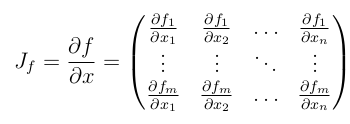
\includegraphics[width=7cm]{sections/imgs/39.png}
\end{center}
Example:
\begin{center}
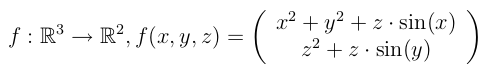
\includegraphics[width=7cm]{sections/imgs/40.png}
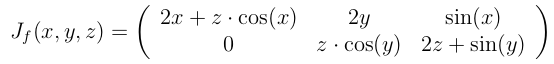
\includegraphics[width=7cm]{sections/imgs/41.png}
\end{center}

\subsection{Applications in Mathematics}
\subsubsection{Taylor's theorem}
One important usage of the Jacobian is the approximation of a function f in a sufficiently small neighborhood about a point $ x \in \mathbb{R}^{n} $, known as Taylor’s theorem:
\[ f (x + \delta x) \approx f (x) + \frac{\partial f}{\partial x} \cdot \delta x =  f (x) + \mathbf{J}_{f} (x) \cdot \delta x \]

\subsubsection{Multi-dimensional chain rule}
\[ (f \circ g)^{'} (t) = f^{'} (g (t)) g^{'} (t) \] 

The scalar derivatives are being replaced with Jacobi matrices: 
\[\mathbf{J_{a}} (f \circ g) = \mathbf{J}_{g (\mathbf{a})} (f) \mathbf{J_{a}} (g), \quad \mathbf{a} = (x,y,z)^T \]

\subsection{Jacobian as the Derivative of the Position Representation (Differential motion)}
We're often not only interested in position and orientation themselves, but also how they are affected by changes in robot parameters $\delta \theta$. These changes can be either small changes (leading to approximation via Taylor’s theorem), or velocities (specified as derivatives of a joint trajectory).

\begin{center}
	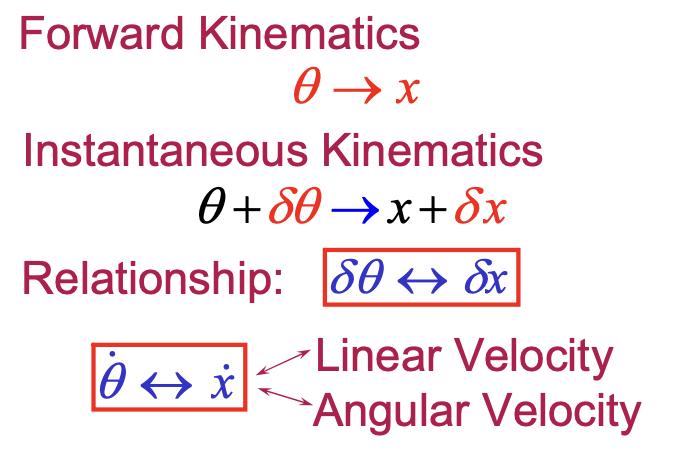
\includegraphics[width=6cm]{sections/imgs/4_pos_velocities.png}
\end{center}
We assume that we are given a position description of a robot coordinate system in form of a function $f$ (params: joint positions, mapped to 6-dim position and orientation representation). Because this representation could use quaternions, rotation matrices or variants of Euler angle conventions, this leads to different Jacobians.

\begin{center}
	$f: \mathbb{R}^{n} \rightarrow \mathbb{R}^{6}, (x_1 , x_2 , ..., x_{n} \mapsto (y_1 , y_2 ,...,y_{6} ))$
\end{center}

We define joint coordinates $q_i$, which combine revolute and prismatic joints. Then, the Jacobian is obtained from the derivative of the position representation w.r.t. the joint coordinate vector $\frac{\partial f(q)}{\partial q}$.

\begin{center}
	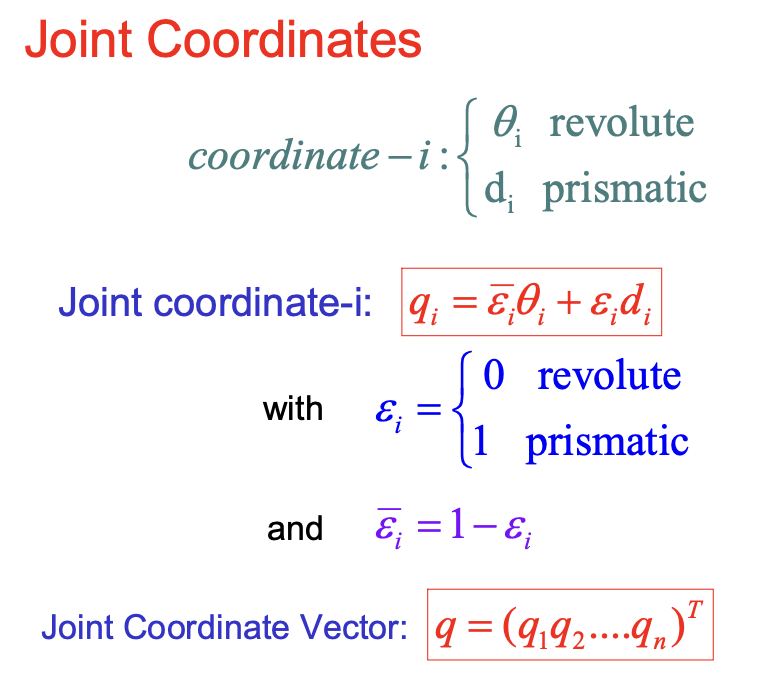
\includegraphics[width=6cm]{sections/imgs/4_joint_coordinates.png}
	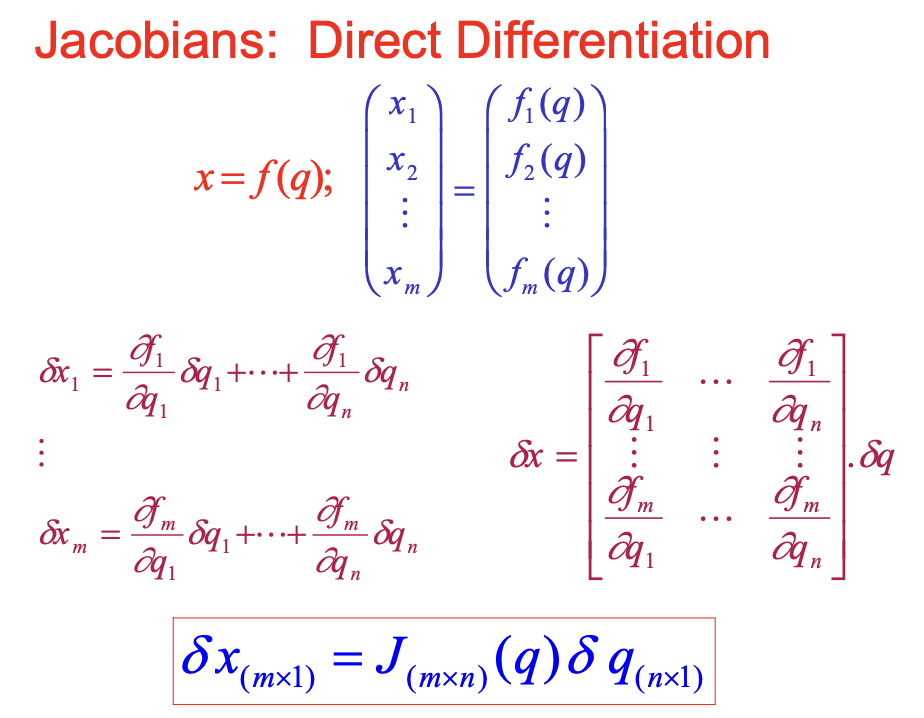
\includegraphics[width=7cm]{sections/imgs/4_direct_diff.png}
\end{center}

An example from the Stanford Lecture:

\begin{center}
	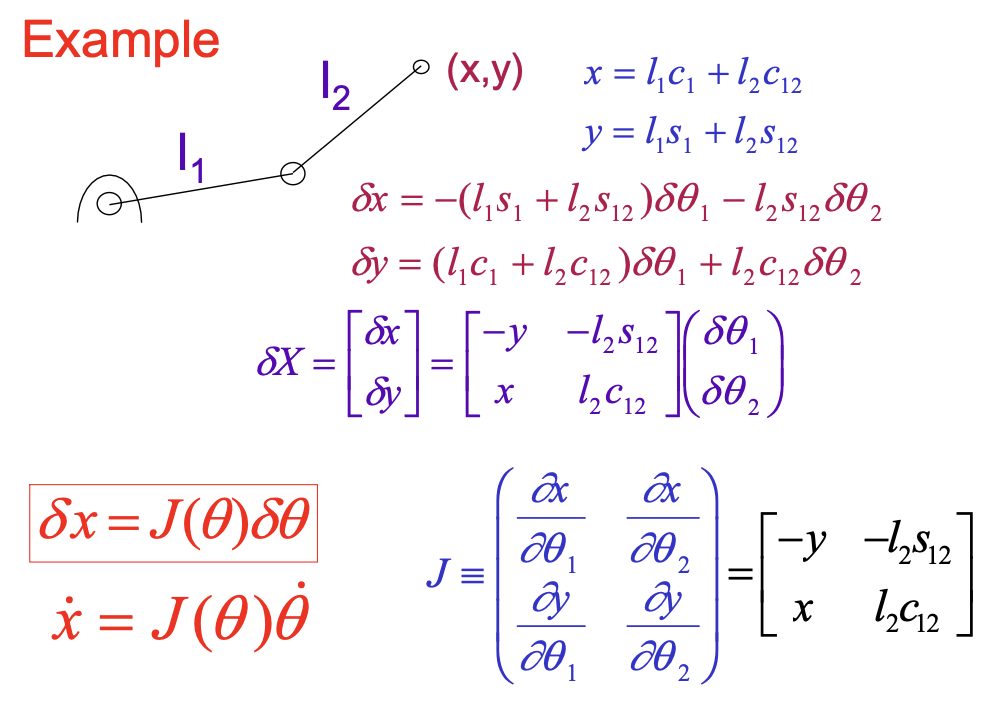
\includegraphics[width=10cm]{sections/imgs/4_position_derivative_example.png}
\end{center}

\textbf{Note that in the TUM lecture material, the joint coordinates are denoted as $\Theta$}. Since the joint angles of a robot must vary over time to cause a motion, the joint positions $ \Theta_{1} , \Theta_{2} , ..., \Theta_{n} $ depend on time $ t $. However, we usually omit the $t$ in $ \Theta_{i} (t) $. All in all:

\[ \Theta (t): \mathbb{R} \rightarrow \mathbb{R}^{n}, t \mapsto (\Theta_{1} (t)  , \Theta_{2} (t)  , ..., \Theta_{n} (t))^T  \]

Then, the position representation at time $ t $ is written as follows:
\[ f (\Theta (t)), \qquad \mathbb{R} \rightarrow \mathbb{R}^{6}\]

\subsubsection{Craig's derivation of rotational velocities}
He uses a rotation-vector $ \boldsymbol{v} \in \mathbb{R}^{3} $ that represents the axis of rotation through its direction and the angle of rotation through its length $ \left| \boldsymbol{v} \right| $. The $\boldsymbol{0}$ vector represents the identity.

Differentiating rotation vectors $ \boldsymbol{v} $ w.r.t joint angles leads exactly to the angular velocity vectors $ \boldsymbol{\omega} $ that are used in his book.
 
\subsection{Jacobians and Velocities}
The Jacobian has the nice property of defining a relation between linear and angular velocities in joint space and velocities in cartesian space (for example of the end-effector). Here, we are interested in derivative of the position representation $ f $ w.r.t. time. 

In analogy to the position representation with small changes in the link coordinates, the same Jacobian connects the derivative of the position representation w.r.t. time and the angular and linear velocities of the joint coordinates:

\begin{center}
	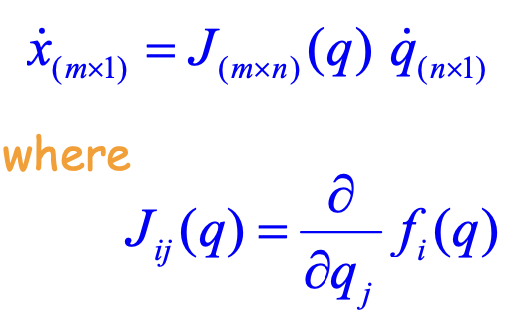
\includegraphics[width=3.5cm]{sections/imgs/4_velocity_derivative.png}\\
\end{center}

The proof written in the notation of the TUM lecture (the first line applies the chain rule):
\begin{align*}
	 \dot{f} = \frac{\partial f}{\partial t} &= \frac{\partial f}{\partial (x_1 , ..., x_{n})} \frac{\partial \Theta}{\partial t} \\
								   &= \frac{\partial f}{\partial (x_1 , ..., x_{n})} \left( \frac{\partial \Theta_1}{\partial t} , \frac{\partial \Theta_{2} }{\partial t},..., \frac{\partial \Theta_{n}}{\partial t} \right)^T \\
								   &= J \cdot \dot{\Theta}
\end{align*}

The individual components of $f$ are the derivative the the position $\dot{x}_P$ and of the orientation $\dot{x}_R$ and are related to the joint coordinates by individual Jacobians:

\begin{center}
	$\left[\begin{array}{c}
	\dot{x}_P \\
	\dot{x}_R \\
	\end{array}\right]_{6 \times 1}=\left[\begin{array}{l}
J_{x_P} \\
J_{x_R}
\end{array}\right]_{6 \times n} \left[\begin{array}{c}
	\dot{\Theta}_{1} \\
	... \\
	\dot{\Theta}_{n}
	\end{array}\right]_{n \times 1}=J_{6 \times n}\left[\begin{array}{c}
	\dot{\Theta}_{1} \\
	... \\
	\dot{\Theta}_{n}
	\end{array}\right]_{n \times 1}$
\end{center}

Keep in mind that the Jacobian depends on the following circumstances:
 \begin{itemize}
	\item How are positions/orientations represented? A Jacobian that is based on cartesian coordinates will look different than one based on Euler angles. This following images shows the possible representations of position and orientation:
	\[\centering 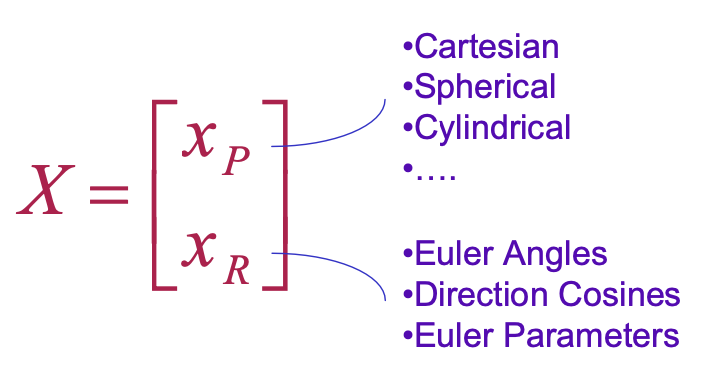
\includegraphics[width=4cm]{sections/imgs/4_X_pos_orientations.png}\]
	\item What is the reference coordinate system for the Jacobian?
	\item How is the current joint configuration?
 \end{itemize}

\textit{Note that for this reason, the Stanford Lecture distinguishes between a Jacobian $J_x$ for the particular representation used in $X$ and a basic Jacobian $J_0$.} These two matrices are related by a matrix $E$ that relates the linear velocity to the position representation and the angular velocity to the orientation representation.

\begin{center}
	$\begin{aligned}
&\dot{x}_{P}=E_{P}\left(x_{P}\right) v \\
&\dot{x}_{R}=E_{R}\left(x_{R}\right) \omega
\end{aligned}$
\end{center}

Herein, $\dot{x}_{P}$ and $\dot{x}_{R}$ are the derivatives of $f$ w.r.t. time and and $v$ and $\omega$ are the linear and angular velocity (these do not match $\dot{x}_{P}$ and $\dot{x}_{R}$ for certain representations!). The following figure shows how the Jacobian and the basic Jacobian are related:

\begin{center}
	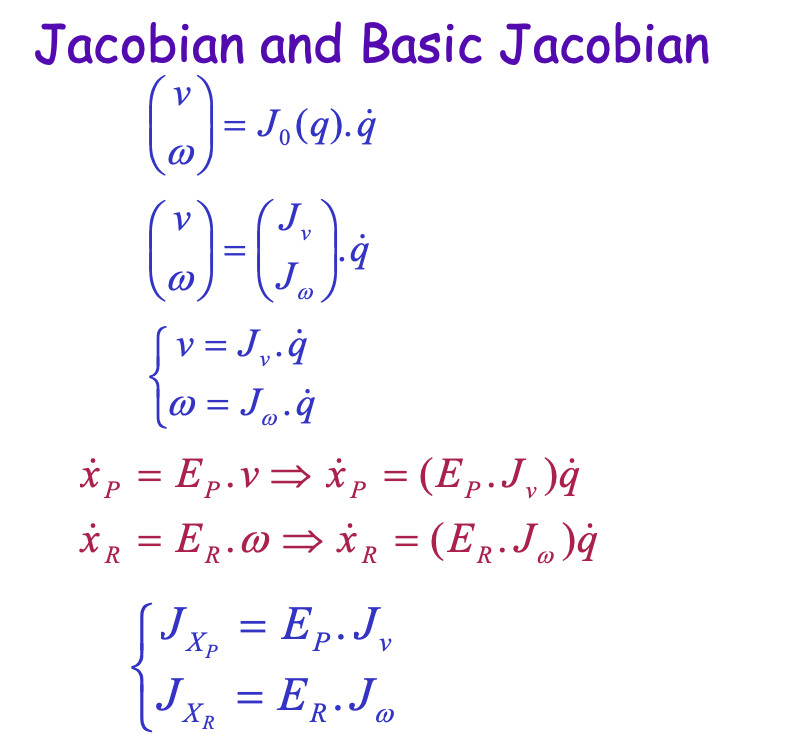
\includegraphics[width=7cm]{sections/imgs/4_jacobian_and_basic_jacobian.png}
	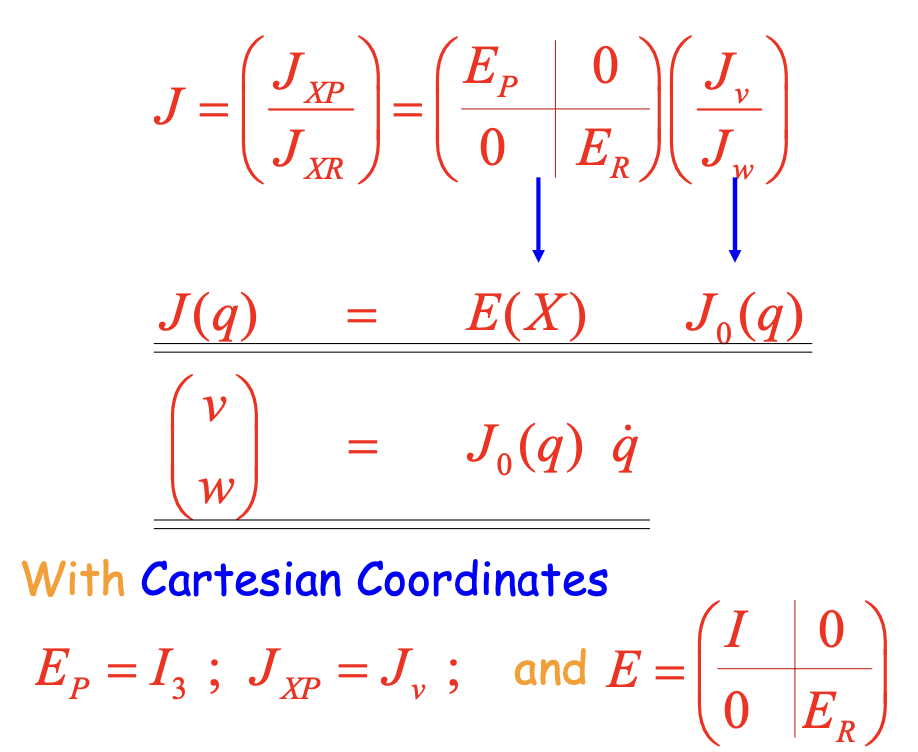
\includegraphics[width=8cm]{sections/imgs/4_x_basic_jacobian_relation.png}
\end{center}

Usually, we want to know $v$ and $\omega$ and derive them from the third equation on the right side of the figure above.

 
\subsection{Velocities}

Linear velocities are always measured in a specific coordinate frame, e.g. the velocity of point $p$ measured in frame $\{A\}$ w.r.t. frame $\{B\}$:

\begin{center}
	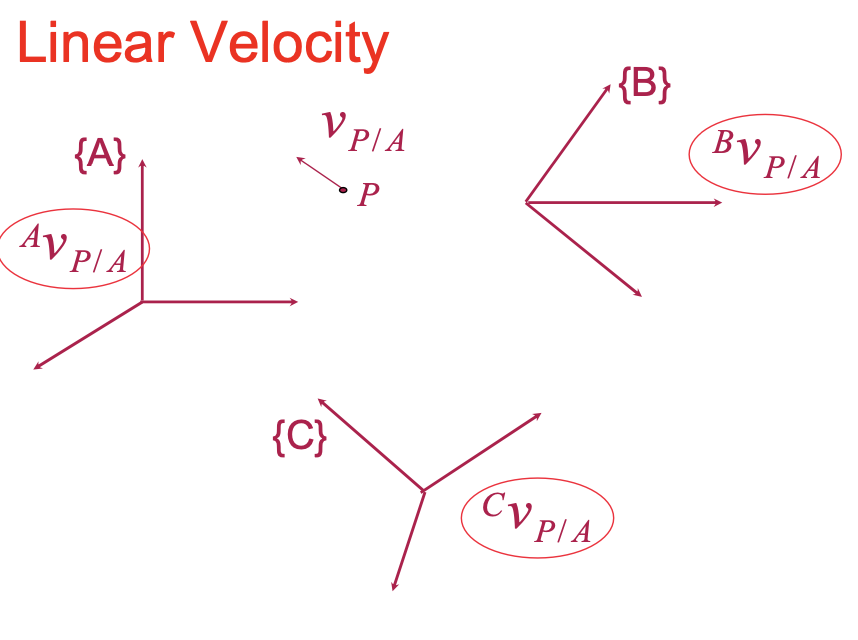
\includegraphics[width=6cm]{sections/imgs/4_linear_velocity.png}
	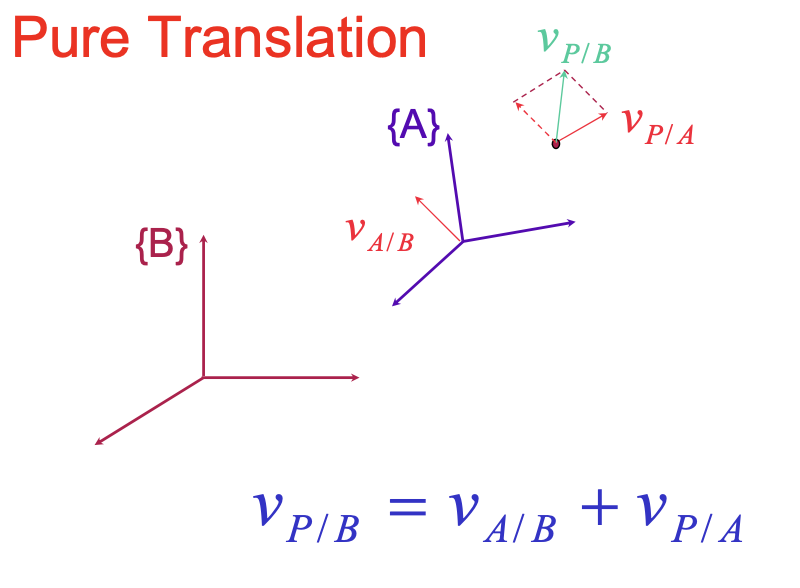
\includegraphics[width=6cm]{sections/imgs/4_pure_translation.png}
\end{center}

The linear velocity from rotational motion derives from the cross product of the angular velocity with the points vector, as seen in the left figure below. When combining linear and angular velocities, one must make sure to express them w.r.t. the correct coordinate frame, hence the right figure.

\begin{center}
	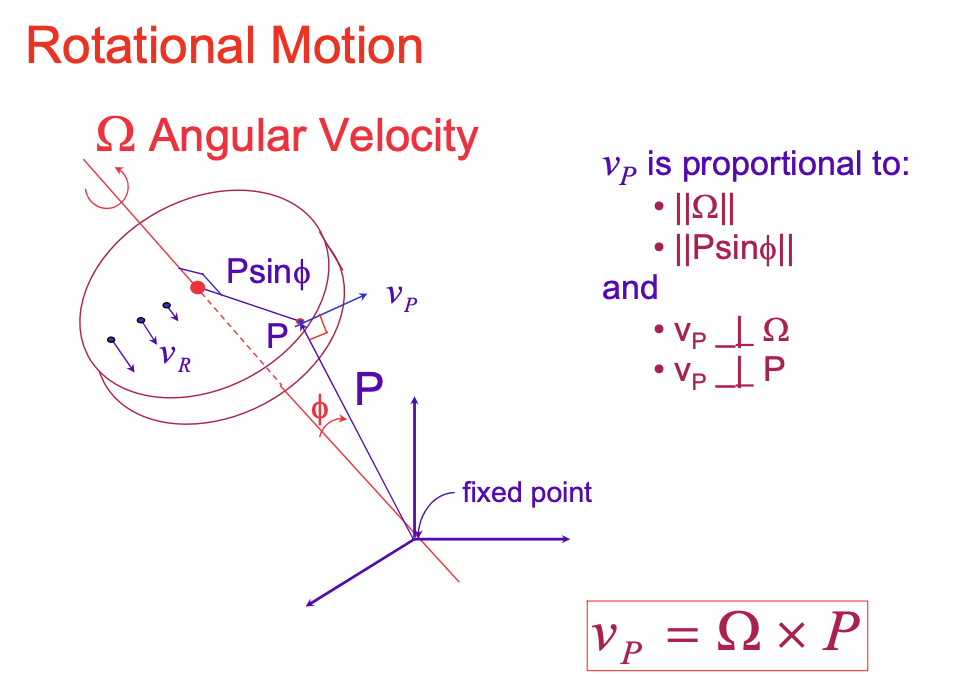
\includegraphics[width=7cm]{sections/imgs/4_rotational_motion.png}
	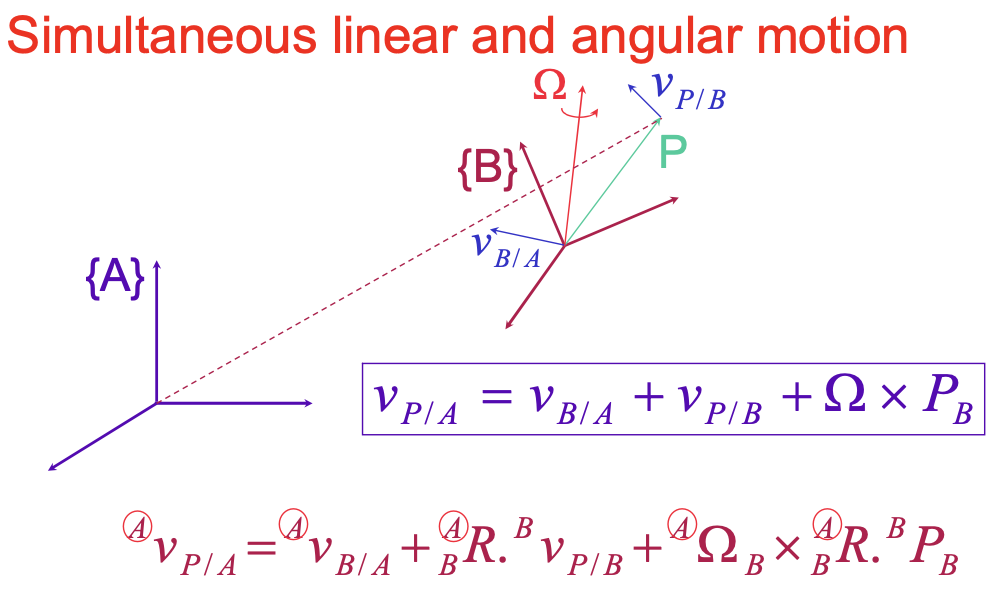
\includegraphics[width=8cm]{sections/imgs/4_sim_lin_and_angular_motion.png}
\end{center}

With these concepts, the angular and linear velocities in robot joints are propagated from the base frame to the end-effector frame.

\begin{minipage}[c]{0.5\textwidth}
$
\begin{aligned}
	&\ {}^{i+1} v_{i+1} = {}^{i+1}_{i} R ({}^{i} v_{i} + {}^{i} \omega_{i} \times {}^{i} P_{i+1}) + \dot{d}_{i+1} \cdot {}^{i+1} \hat{Z}_{i+1}\\
	&\ {}^{i+1} \omega_{i+1} = {}^{i+1}_{i} R \cdot {}^{i} \omega_{i} + \dot{\Theta}_{i+1} \cdot {}^{i+1} \hat{Z}_{i+1}\\
\end{aligned}
$
\begin{center}
	$\dot{d}_{i+1}$ or $\dot{\Theta}_{i+1}$ for prismatic/ revolute joints (scalars).
\end{center}

\end{minipage}
\hfill
\begin{minipage}[c]{0.5\textwidth}
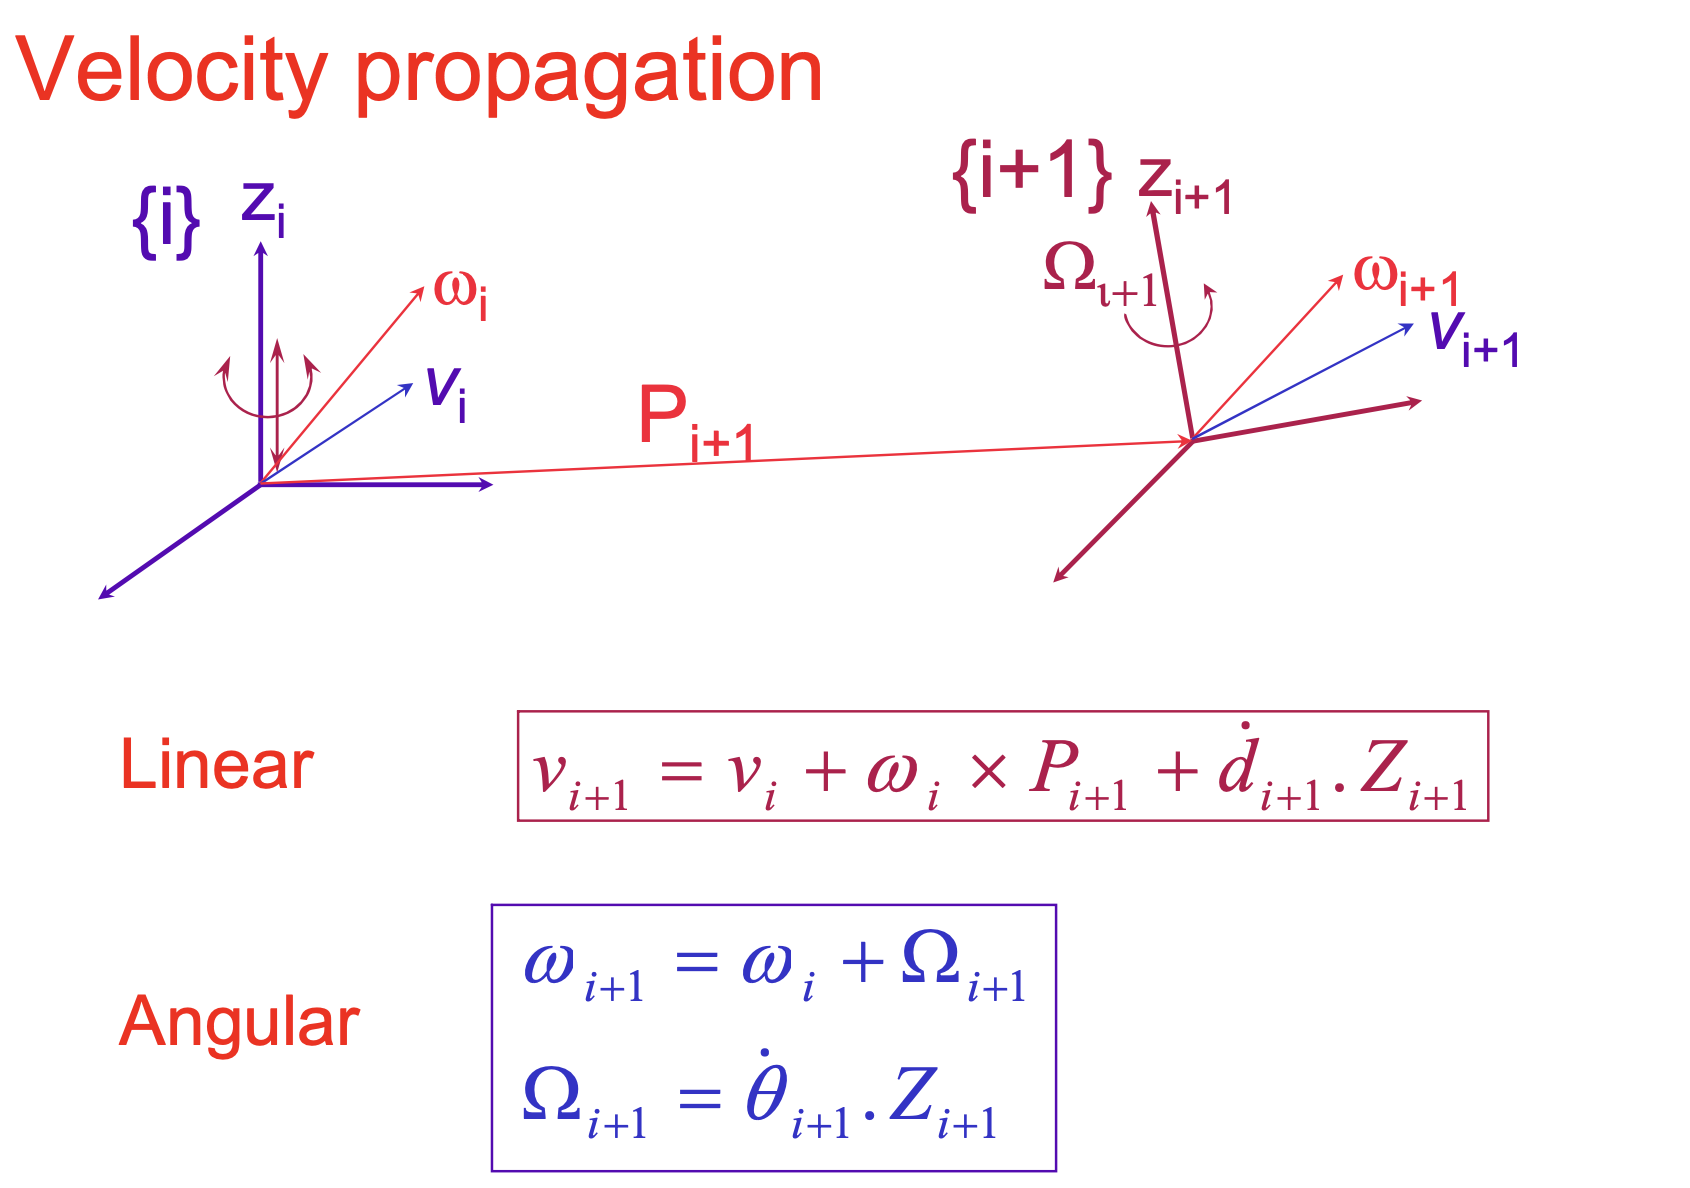
\includegraphics[width=9cm]{sections/imgs/4_velocity_propagation.png}\end{minipage}

The linear velocity w.r.t. frame $i+1$ is the sum of the linear velocity of frame $i$, the cross product of the angular velocity of frame $i$ with the distance between the two frames and the joint velocity along $\hat Z_{i+1}$ if $i+1$ is a prismatic joint (otherwise, $\dot{d}_{i+1}=0$). ${}^{i+1}_{i} R$ maps the vectors from from $i$ to frame $i+1$.\\
The angular velocity w.r.t. frame $i+1$ is composed of the  angular velocity of of the previous frame plus the angular velocity around $\hat Z_{i+1}$ if $i+1$ is a revolute joint.\\

The expressions for the linear and angular velocities at a given frame $n$ can be used to determine the full Jacobian indirectly:
\[ {}^{n} J \dot{\Theta} = \begin{pmatrix} {}^{n} v_n \\ {}^{n} \omega_{n} \end{pmatrix} \]
where the shape of the Jacobian on the left hand side can be determined from the shape of the linear-angular velocity vector on the right hand side (by factoring out the derivatives of the joint coordinates). Herein, the expressions for ${}^{n} v_n$ and ${}^{n} \omega_{n}$ are obtained from the two equations above.

An example for this is found in \href{https://youtu.be/fwHc0a8DMQ0?t=4040}{Lecture 6 of the Stanford course}.

\subsection{Explicit Form}

This section details how one can easily \textit{see} the Jacobian matrix in a manipulator. The next figure shows a manipulator with prismatic and revolute joints:
\\

\begin{minipage}[c]{0.5\textwidth}
	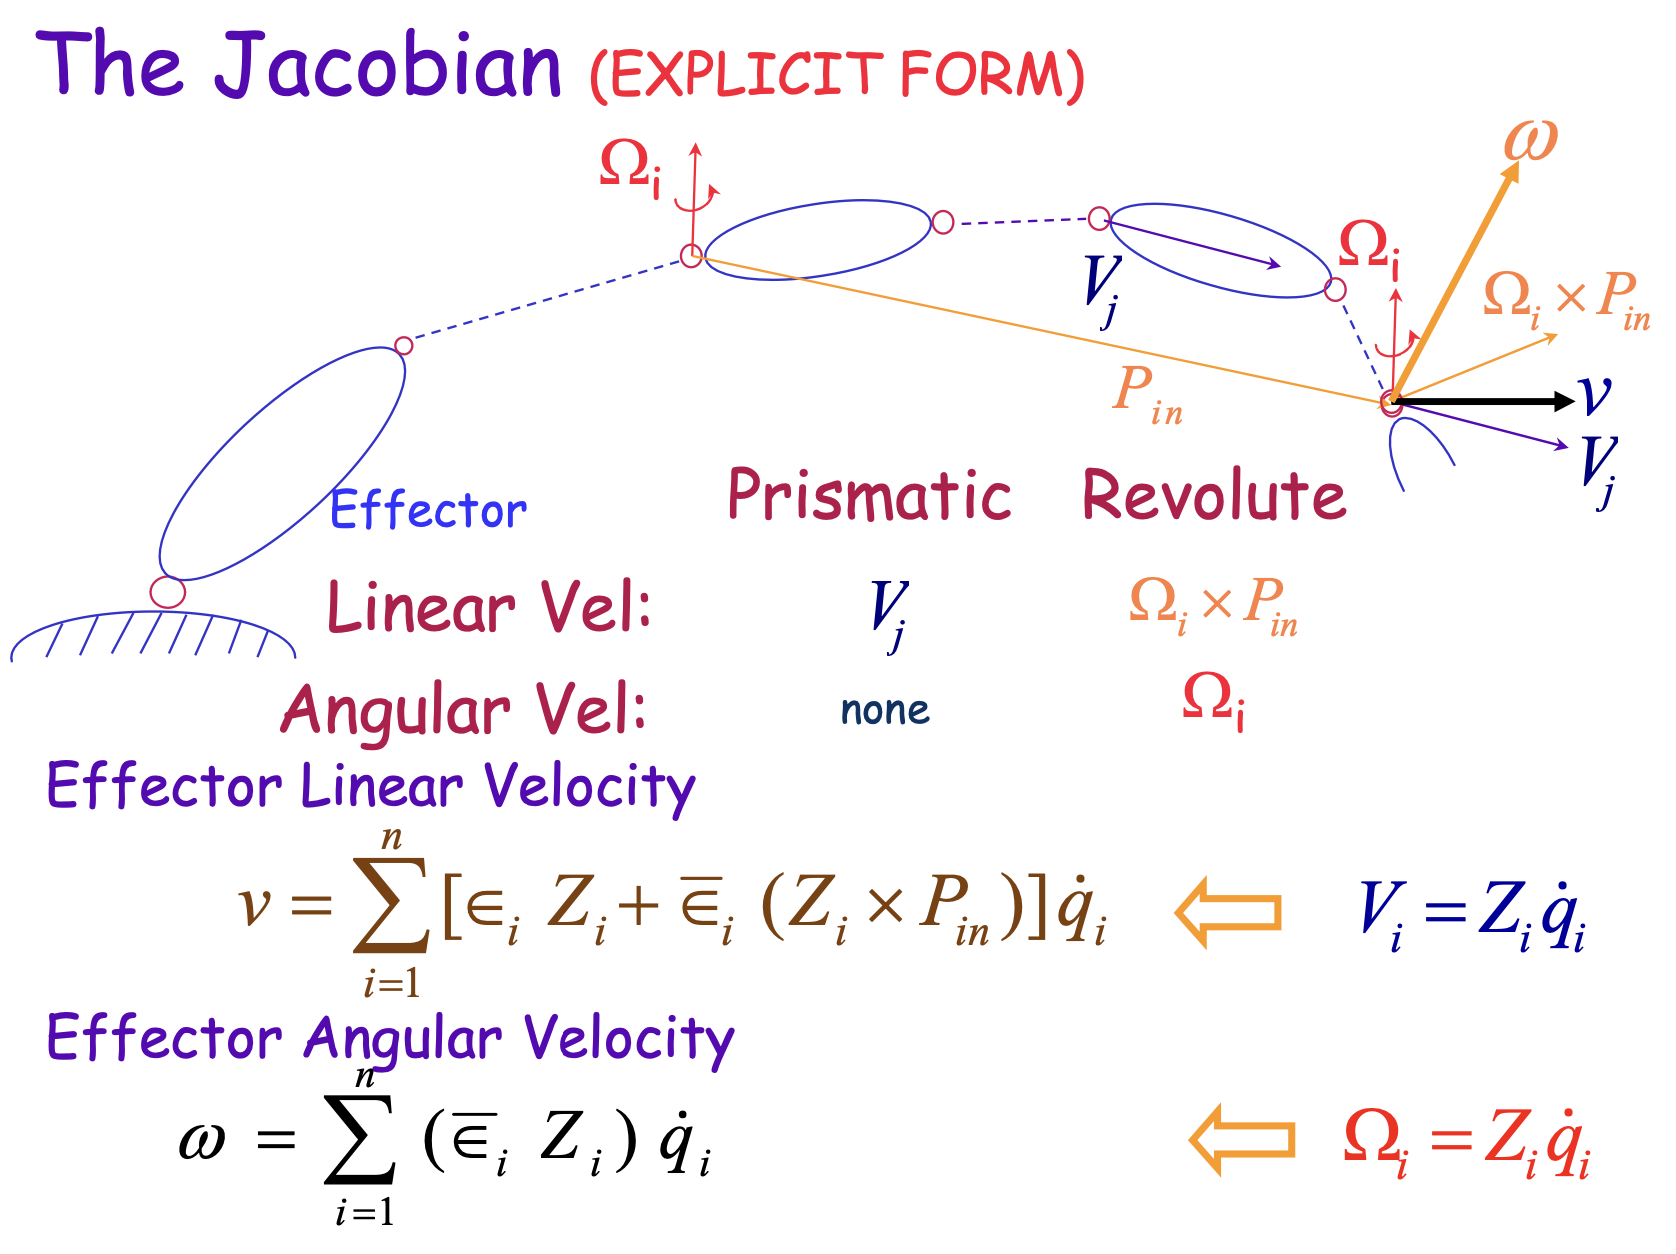
\includegraphics[width=9cm]{sections/imgs/4_jacobian_explicit_form.png} 
\end{minipage}
\hfill
\begin{minipage}[c]{0.5\textwidth}
	\begin{center}
	\begin{enumerate}
		\item The impact of each joint type on the end-effector is given in the table.
		\item The linear/ angular velocity of prismatic/ revolute joints is a function of the joints' $Z_i$ axes and joint coordinates $q_i$ ($\dot d$ or $\dot \theta$).
		\item The total velocities at the end-effector are the sum over the components from all joints.
	\end{enumerate}
	\end{center}
\end{minipage}
\\

In order to derive the Jacobian, we need to factor out the $q$s:\\

\begin{minipage}[c]{0.5\textwidth}
	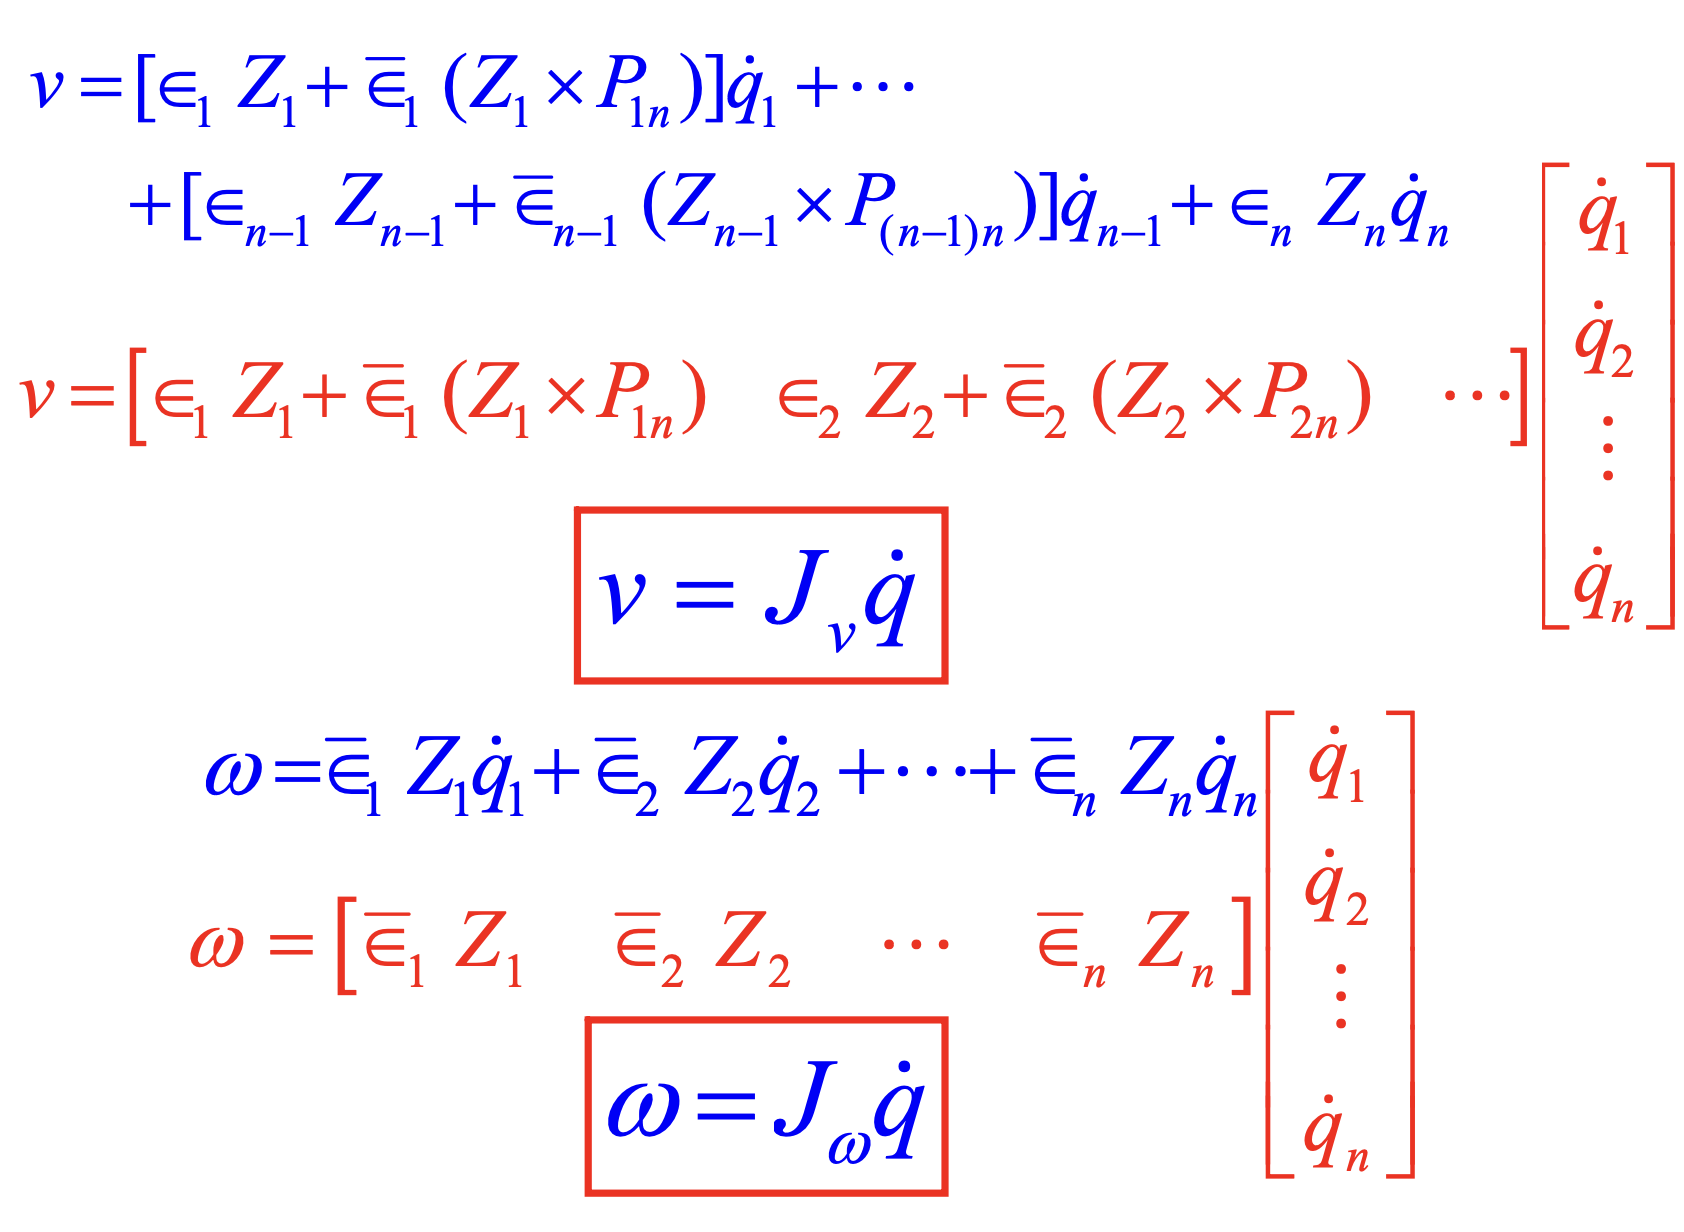
\includegraphics[width=9cm]{sections/imgs/4_jacobian_explicit_form_2.png}
\end{minipage}
\hfill
\begin{minipage}[c]{0.5\textwidth}
	\begin{center}
	\begin{enumerate}
		\item Linear velocity: Each column in $J_v$ is the joint axis if the joint is prismatic or the cross product of the axis with the vector connecting the joint to the end-effector if the joint is revolute.
		\item Angular velocity: Each column in $J_\omega$ is the  joint axis if the joint is revolute or the $\boldsymbol{0}$ vector if it is prismatic.
		\item \textit{Note:} We need to express all vectors w.r.t. the frame in which we want to define our Jacobian.
	\end{enumerate}
	\end{center}
\end{minipage}\\

When using cartesian coordinates, we can also obtain $J_v$ directly from the derivative of the forward kinematics (or ``translation'' column in the homogeneous transform) w.r.t. the joint coordinates $q$. This is clearer when looking at the left side of the next figure. \\

The full Jacobian $J$ in some frame then consists of these $J_v$ and $J_\omega$ matrices. In order to express $J$ in reference frame $\{0\}$ we need to multiply every $Z_i$ axis with the the respective mapping ${}^0_i R$, as shown in the next figure. Note that the product ${}^0_i R \ Z_i$ is simply the third column of the rotation matrix! If we have the homogeneous transform, we can just pick the components for our Jacobian!\\

\begin{center}
	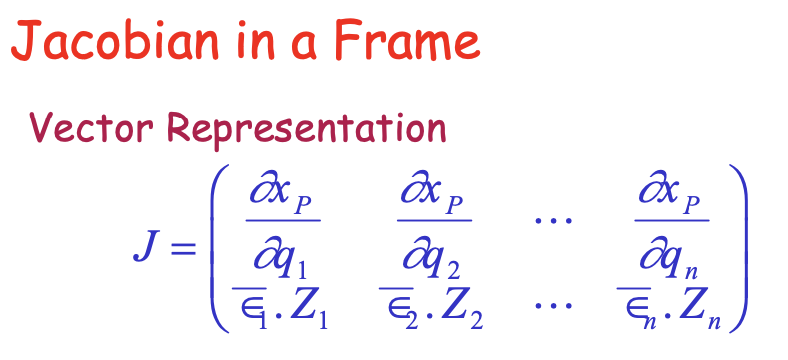
\includegraphics[width=8cm]{sections/imgs/4_jacobian_in_a_frame.png}
	\hfill
	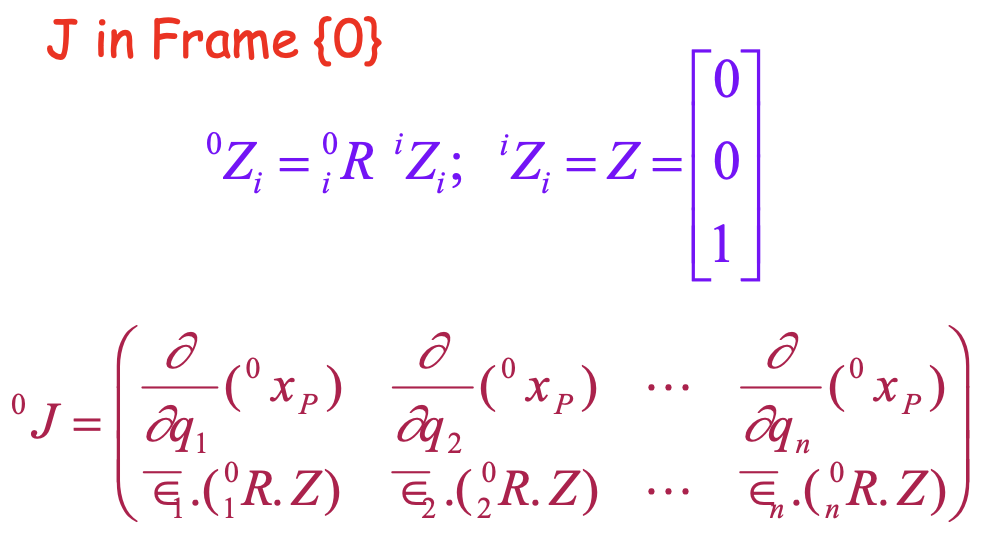
\includegraphics[width=8cm]{sections/imgs/4_J_in_frame_0.png}
\end{center}

In \href{https://youtu.be/6SRTAoyzC6A?t=2235}{lecture 7 of the Stanford Lecture} you can find an example to practice \textit{seeing} the Jacobian.

Finally, these two rules may help (derived in Lecture 8 of the Stanford lecture):
\begin{center}
	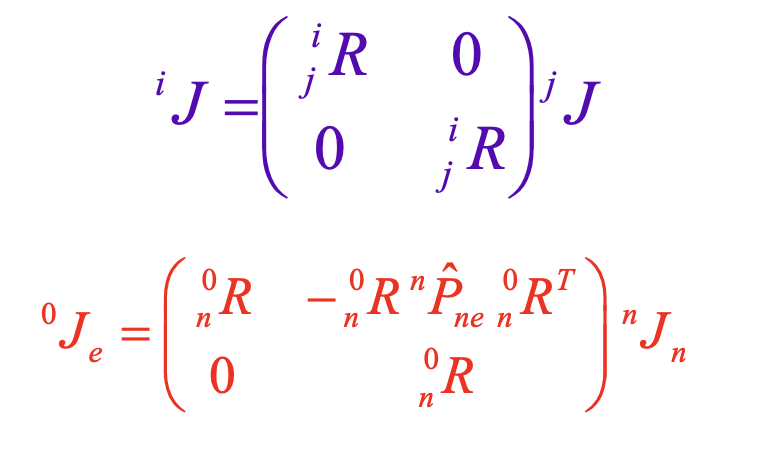
\includegraphics[width=6cm]{sections/imgs/4_jacobian_relate_frames.png}
\end{center}

\subsection{Kinematic Singularity}

If the configuration of the robot manipulator reaches a singularity, the end-effector \textit{locally} loses the ability to move in a direction or to rotate about a direction, e.g. because two axes of revolute joints become collinear (see \href{https://youtu.be/XrNdB4k5kUk?t=575}{this explanation}).

Since the singularity happens, when $Z$ axes are aligned, the Jacobian does not have full rank in these situations (columns become dependant). In this case, the determinant is zero.
\begin{center}
	$
	\begin{aligned}
		 \det(J)&=0 \\
		 \det({}^i J)&=\det({}^j J)\\
		 \det(J)&=\det(J^T J)\ \text{   Trick if $J$ is not square.}
	\end{aligned}
	$
\end{center}
The determinant is the same in every reference frame! We can then find all singular configurations by setting the $\det(J)$ in any reference frame to zero.\\

\begin{minipage}[c]{0.5\textwidth}
	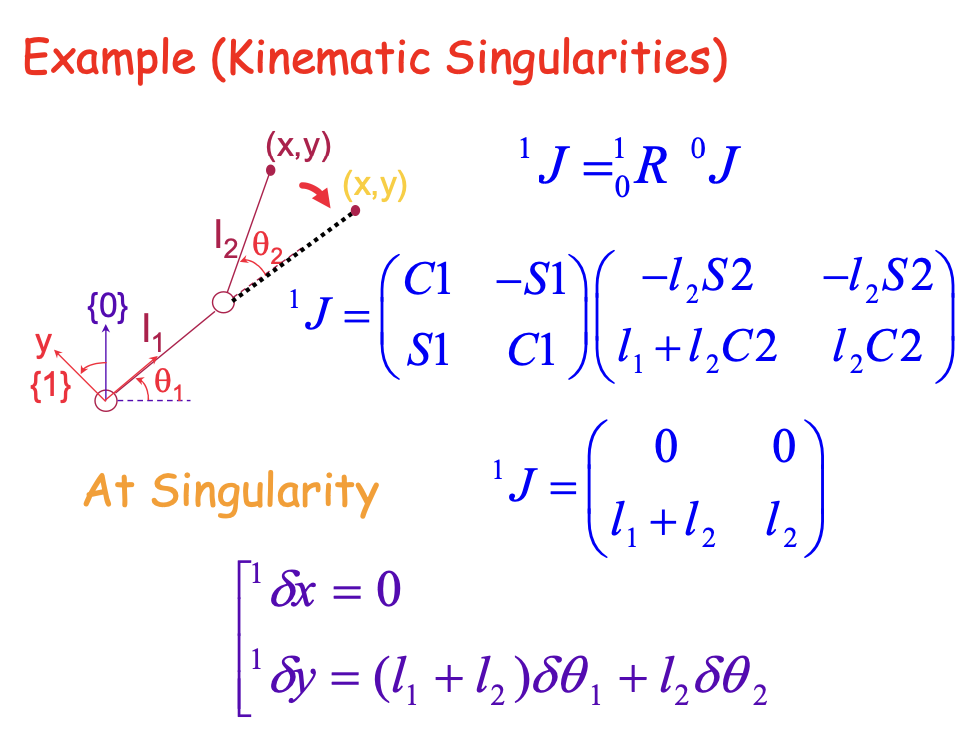
\includegraphics[width=8cm]{sections/imgs/4_kinematic_singularities.png}
\end{minipage}
\hfill
\begin{minipage}[c]{0.5\textwidth}
	\begin{center}
	\begin{enumerate}
		\item When the second joint angle is zero ($\theta_2=0$), the Jacobian in this frame becomes rank 1.
		\item From the relationship $[\delta x, \delta y]^T = J \ \delta\Theta$ follows that no motion in the local $x$ direction is possible. This is a singularity.
	\end{enumerate}
	\end{center}
\end{minipage}\\

\subsection{Jacobian for Approximating very small (``infinitesimal'') Movements}
Taylor's theorem (which states that a function behaves like its derivative in a sufficiently small environment) can be used to approximate how the position of the end effector changes whenever small changes are made to robot parameters. 

The theorem can be used to derive the following: 
\[ \delta x \approx J^{-1} (f (x + \delta x) - f (x))  \]
$ \delta x $ denotes a small change in $ x $, or a small change in the robot parameters. Using this equation, we can relate small changes $ \delta x $ in joint parameters to a small change $ f (x+ \delta x) - f (x) $ in position, and vice-versa.

This is the reason why singular configurations should be avoided: $ J $ becomes ill-conditioned near those, meaning that computed $ \delta x $ might approach infinity.

Singular positions are reached when $ det(J) = 0 $. Using this condition, we can figure out which joint parameters should be avoided.

\subsection{Frame of reference of a Jacobian}
Given a Jacobian in reference system B, the following equation related joint velocities to cartesian and angular velocities.
\[ \begin{pmatrix} {}^{B} v\\ {}^{B} \omega \end{pmatrix} = {}^{B} J (\Theta) \dot{\Theta}\]
And for a Jacobian w.r.t system A:
\[ {}^{A} J (\Theta) \dot{\Theta } = 
	\begin{pmatrix} {}^A_B R & \mathbf{0} \\ \mathbf{0} & {}^A_B R \end{pmatrix} {}^B J (\Theta) \dot{\Theta} \quad \Rightarrow \quad {}^A J (\Theta ) = \begin{pmatrix} {}^A_B R & \mathbf{0} \\ \mathbf{0} & {}^A_B R \end{pmatrix} {}^B J (\Theta)  \]

\subsection{Forces and Torques in Static Manipulators}
This section is based on page 156 of the book, exercise sheet 3 and the 8th lecture of the Stanford course.

In the figure below, two fundamental relations between torque exerted through motion around an axis and the force at a given point are derived.

\begin{center}
	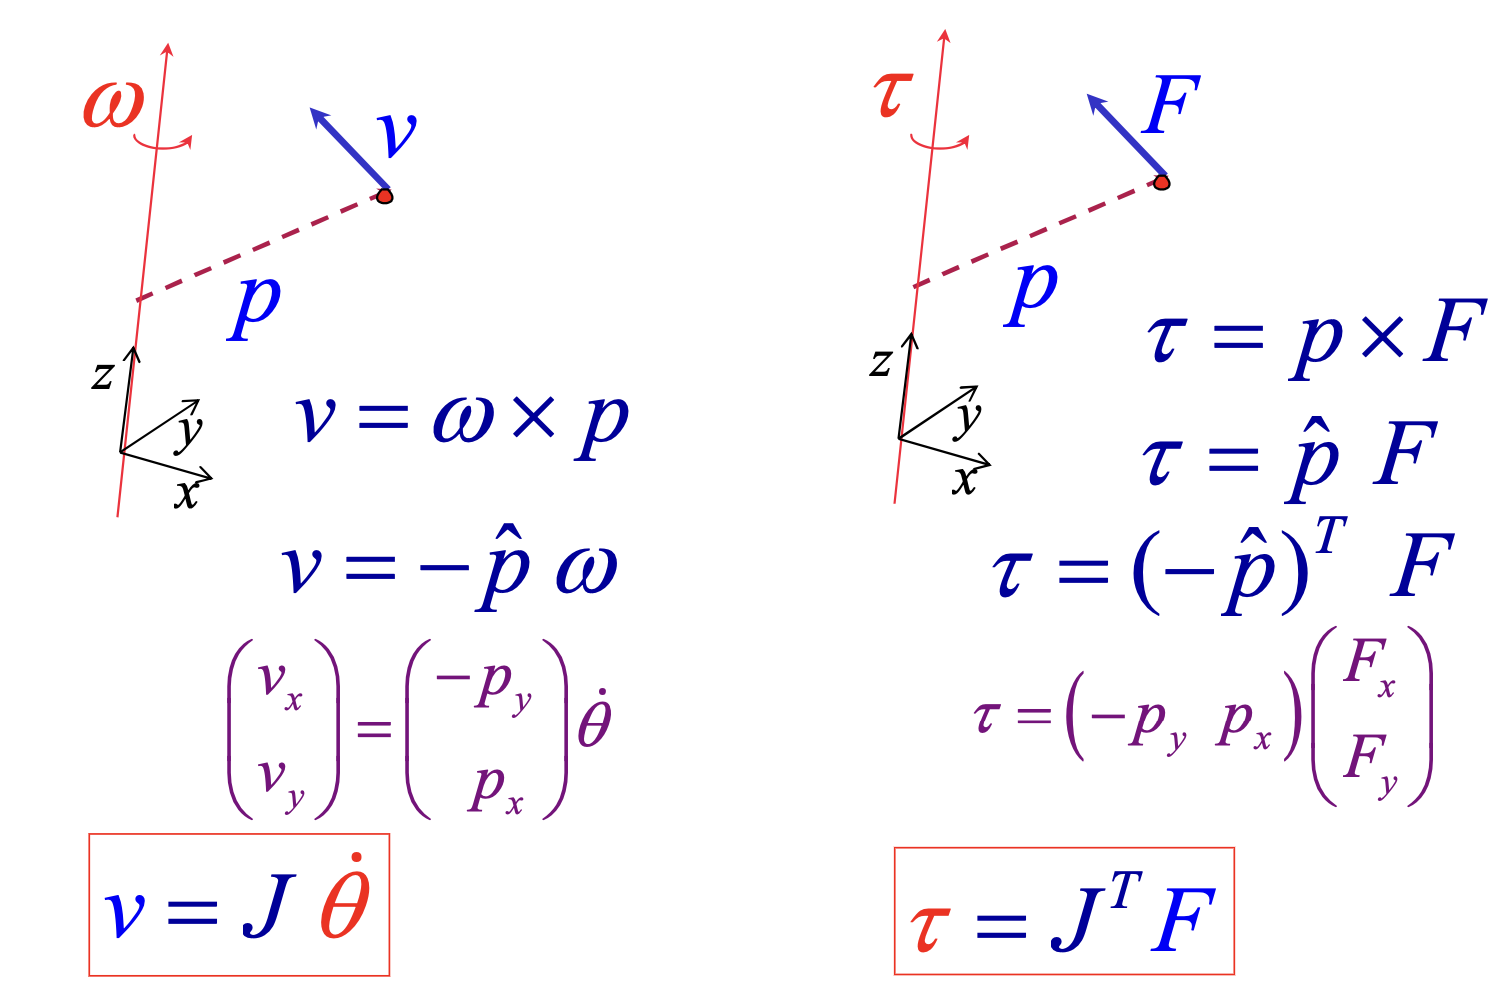
\includegraphics[width=9cm]{sections/imgs/4_force_torque.png}
\end{center}

The linear velocity $v$ is the cross product between $\omega$ and the point vector. $\omega \times p = - p \times \omega$ can be rewritten using the matrix operator $\hat{p}$ that expresses the cross product. In the right part of the figure we use the fact that $\hat{p} = (-\hat{p})^T$. When we calculate the results of the cross products, we are left with the equations in red. It turns out that, while linear and angular velocity are related via the Jacobian, torque is related to force via its transpose.\\

The book derives this equation in another way: in the multidimensional case, work is the dot product of a vector force or torque and a vector displacement:
\[ \mathcal{F} \cdot \delta \mathcal{X} = \tau \cdot \delta \Theta  \]
where $ \mathcal{F} $ is a $6\times1$ cartesian force-moment vector acting at the end-effector, $ \delta \mathcal{X} $ is a $6\times1$ infinitesimal cartesian displacement of the end-effector, $ \tau $ is a $6\times1$ vector of torques at the joints, and $ \delta \Theta $ is a $6\times1$ vector of infinitesimal joint displacements. 

\begin{center}
	$\left(\begin{array}{c}
\tau_{1} \\
\tau_{2} \\
\vdots \\
\tau_{n}
\end{array}\right)=\tau={ }^{A} J^{T A} \mathcal{F}={ }^{A} J^{T}\left(\begin{array}{c}
{}^{A}f \\
{}^{A}n
\end{array}\right)$
\end{center}

The Jacobian transpose maps cartesian forces acting at the hand into equivalent joint torques. When the Jacobian is written with respect to frame $\{0\}$, then force vectors written in $\{0\}$ can be transformed, as follows:
\[ \tau = {}^0 J^T \ {}^0\mathcal{F} \]

If we calculate the static equilibrium for each link in a robot manipulator, we are able to relate the forces and torques at the end effector to the forces and torques at the base. The next figure shows the (reaction) forces $f$ and torques $n$ in each link of the manipulator on the left and the static equilibrium of one link on the right.
\begin{center}
	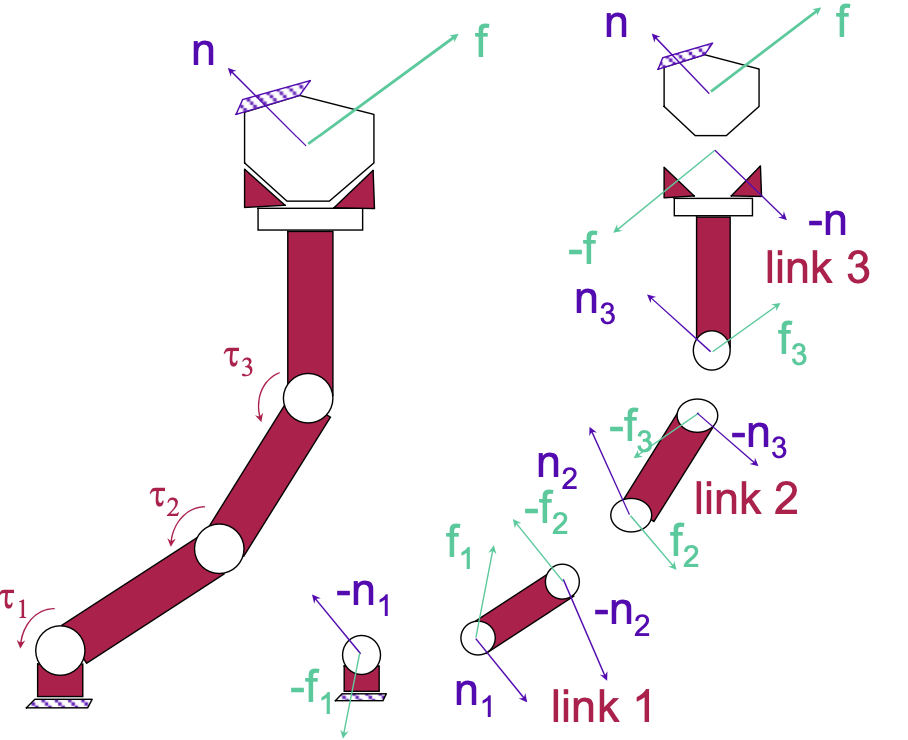
\includegraphics[width=7cm]{sections/imgs/4_propagate_forces_2.png}
	\hfill
	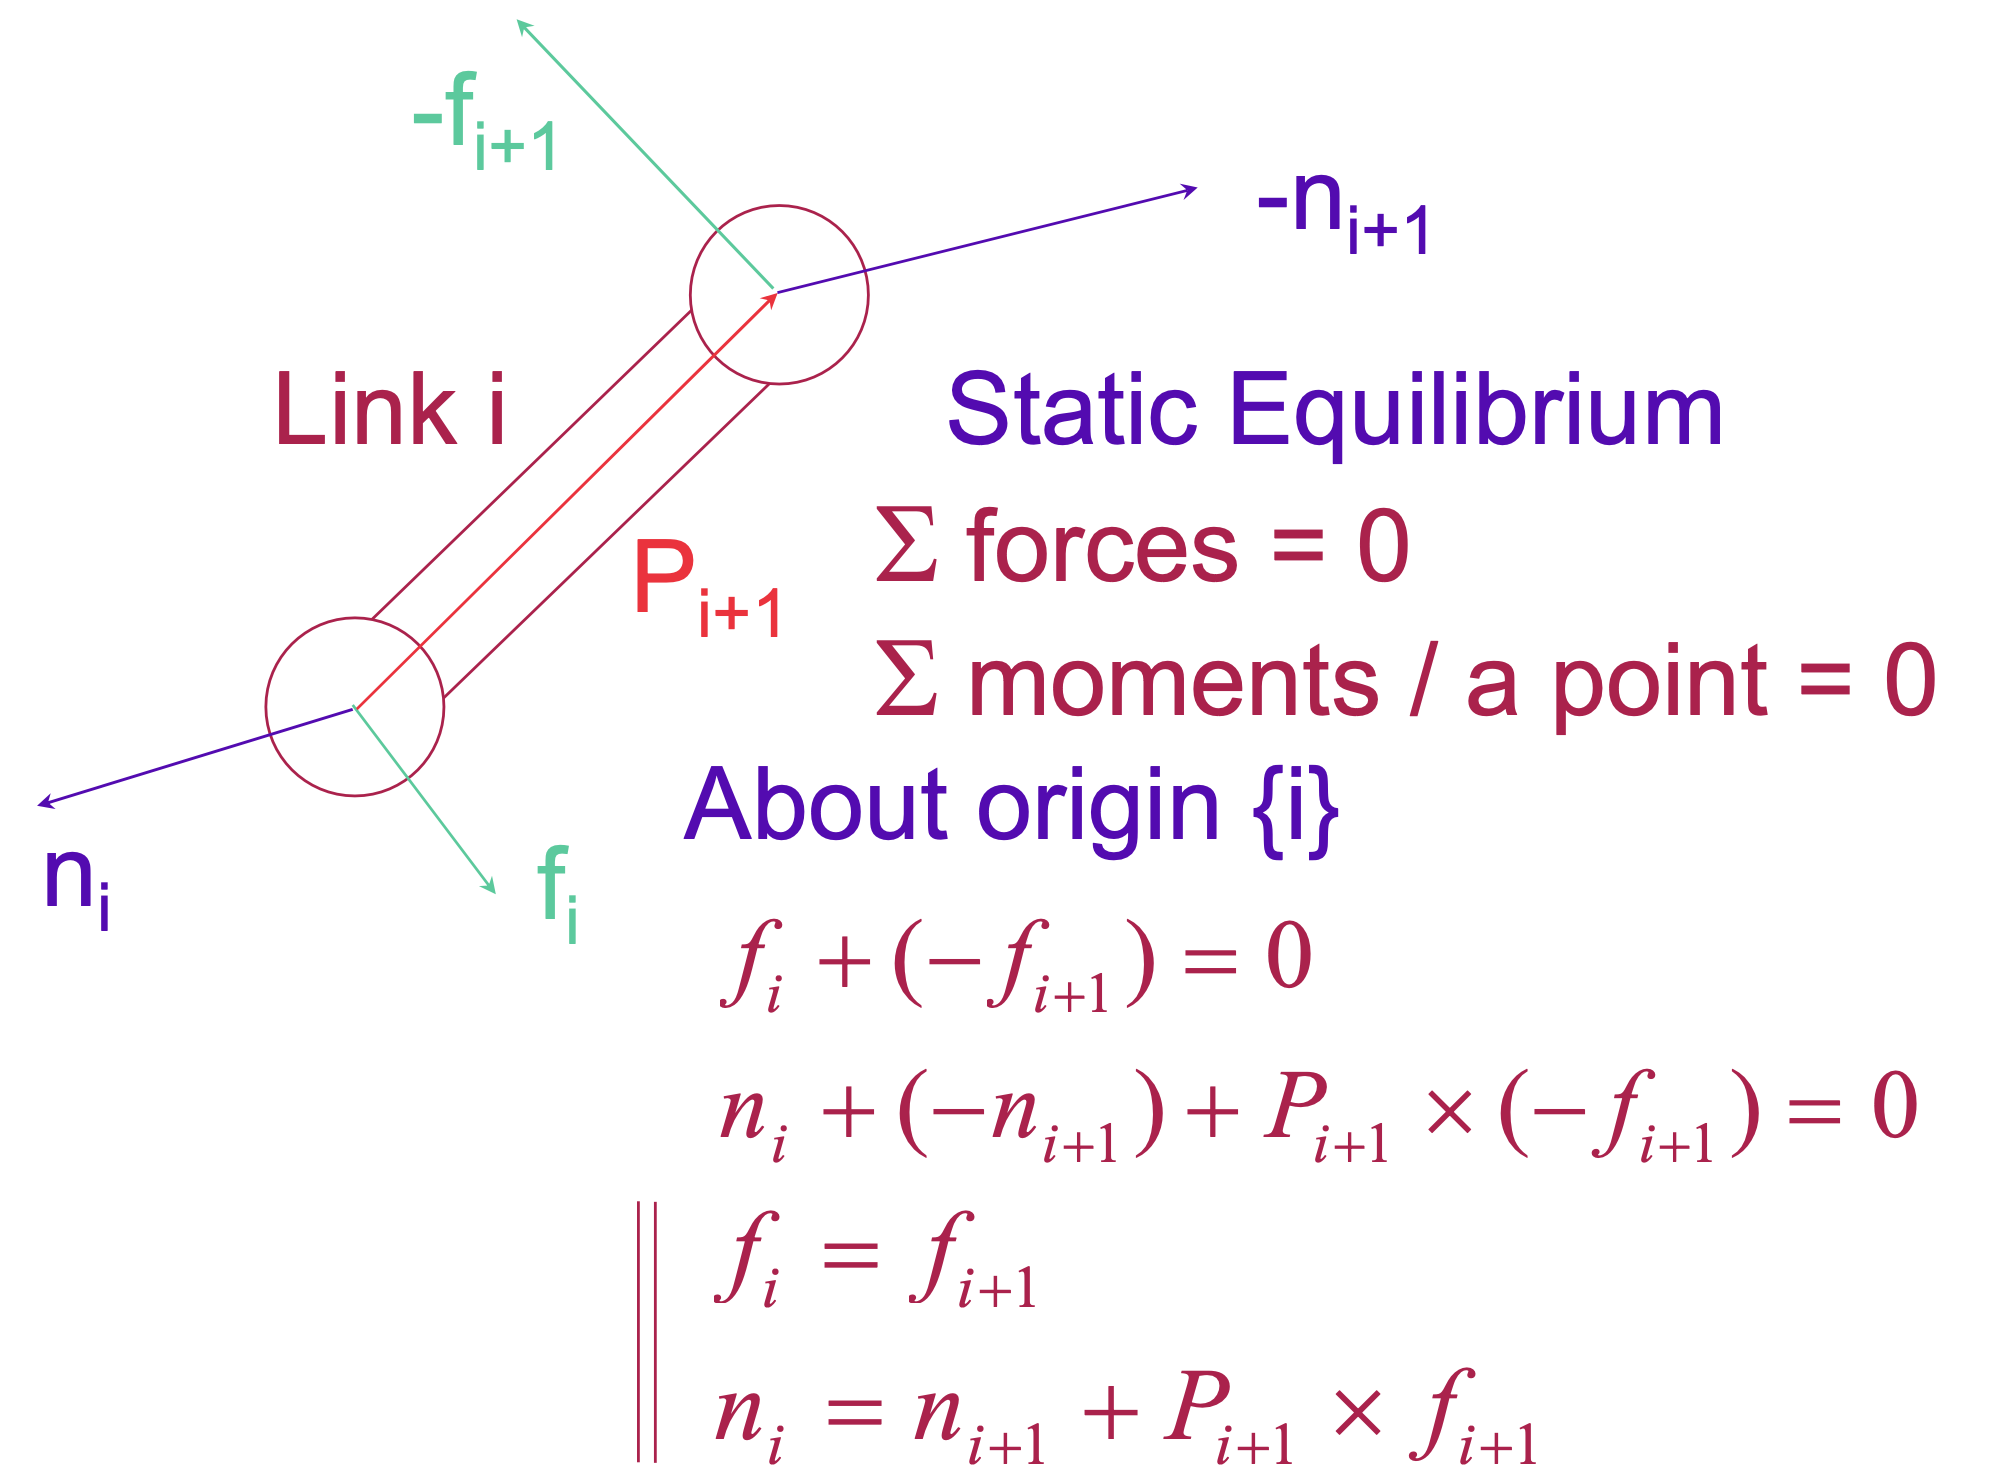
\includegraphics[width=9cm]{sections/imgs/4_propagate_forces.png}
\end{center}

We can then propagate the forces $f_i$ and torques $n_i$ acting on each link from the end-effector to the base:

\begin{center}
	$\begin{aligned}
	&{ }^{i} f_{i}={ }_{i+1}^{i} R \cdot{ }^{i+1} f_{i+1} \\
	&{ }^{i} n_{i}={ }_{i+1}^{i} R \cdot{ }^{i+1} n_{i+1}+{ }^{i} P_{i+1} \times{ }^{i} f_{i}
	\end{aligned}$
\end{center}

The torque that is exerted on prismatic/ revolute joins is given from the projection (inner product) on the joint axis, as shown in the next figure:

\begin{minipage}[c]{0.5\textwidth}
	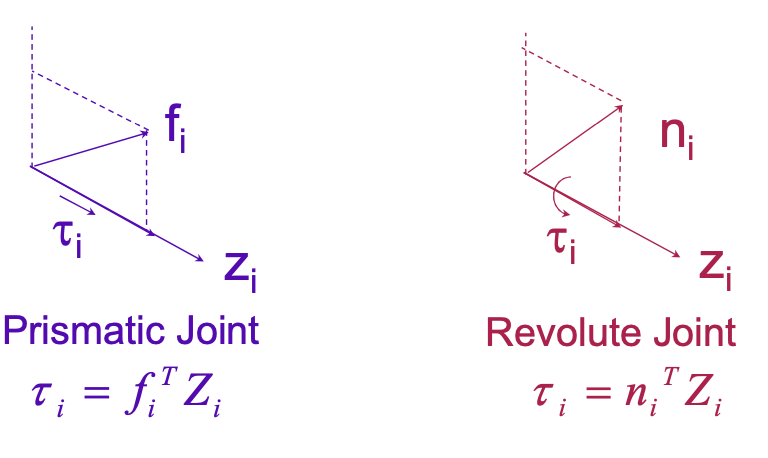
\includegraphics[width=8cm]{sections/imgs/4_prismatic_revolute_torque.png}
\end{minipage}
\hfill
\begin{minipage}[c]{0.5\textwidth}
\begin{center}
$\begin{aligned}
&\tau_{i}={ }^{i} n_{i}^{\mathrm{T} i} Z_{i}={ }^{i} n_{i}^{\mathrm{T}}\left(\begin{array}{l}
0 \\
0 \\
1
\end{array}\right) \\
&\tau_{i}={ }^{i} f_{i}^{\mathrm{T} i} Z_{i}={ }^{i} f_{i}^{\mathrm{T}}\left(\begin{array}{l}
0 \\
0 \\
1
\end{array}\right)
\end{aligned}$
\end{center}

\end{minipage}

The quantities $\tau_i$ thus specify the amount of torque resp. force that is affecting the joint, and thus the amount of torque resp. force that the robot should counteract in order to remain static. The joint torques/forces $\tau_i$ are 1-dimensional quantities.


\newpage
\section{Robot Dynamics}

The field of analytical dynamics, or more briefly dynamics, is concerned with the relationship between motion of bodies and its causes, namely the forces acting on the bodies and the properties of the bodies (particularly mass and moment of inertia) influencing that movement. This is in contrast to kinematics, where we were not concerned with the physical phenomena causing robot movement, but only with the movement itself.

We want to come up with equations of motion for any nDOF system, which express the force require to cause motion. The expression should have the form $ \dot{q} = f (q,t)$\\
We can use it to choose an appropriate controller that will put our dynamical system in a desired state.
This section is based on \href{https://www.youtube.com/watch?v=o3Xx3vi6qzo&list=PL65CC0384A1798ADF&index=12}{Lecture 11} and covered in exercise 4.

\subsection{Rigid Body Dynamics}
\begin{center}
	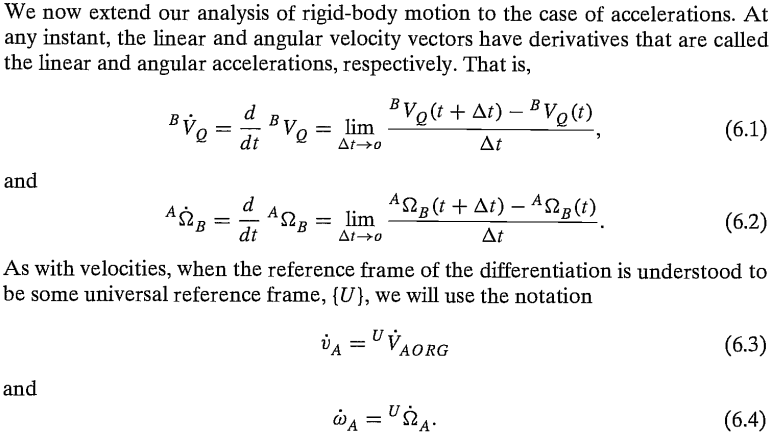
\includegraphics[width=14cm]{sections/imgs/29.png}
\end{center}

\subsection{Newton-Euler Method}
Overall, the purpose of the Newton-Euler-Method is determining the joint torques $\tau$ that are required to achieve a desired motion of the robot. More specifically, if we have a joint trajectory $\Theta (t)$ that describes the positions and velocities for a certain trajectory of the robot, then the Newton-Euler method will allow us to compute corresponding $\tau (t)$ that will, in an ideal world (no friction or other disturbances for the moving robot), cause the robot to carry out the desired trajectory.

\subsubsection{Newton's equation}
A rigid body's center of mass is accelerating with $ \dot{v}_{c} $ when the force $ F $ acts on it. The acceleration is given by
\[ F = m \dot{v}_{c} \]
\begin{center}
	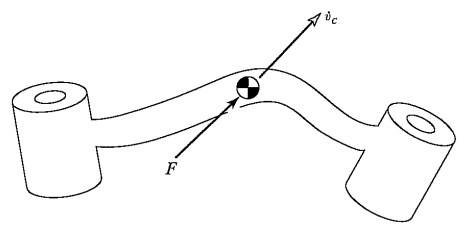
\includegraphics[width=6cm]{sections/imgs/36.png}
\end{center}

\subsubsection{Euler's equation}
The rigid body in the image below rotates with angular velocity $ \omega $ and with angular acceleration $ \dot{ \omega} $. Then, the moment $ N $, which acts on the link is:
 \[ N = {}^{C} I \dot{\omega } + \omega \times {}^{C} I \omega \]
where $ {}^{C} I $ is the inertia tensor that is computed with respect to the center of mass in frame $C$, a $3\times3$ matrix that describes the distribution of masses in a link. \begin{center}
	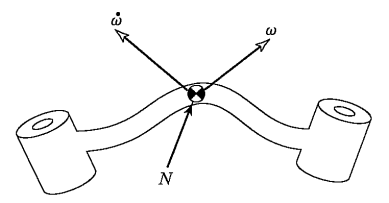
\includegraphics[width=6cm]{sections/imgs/37.png}
\end{center}

\subsubsection{Linear acceleration}
The linear acceleration is the derivative of the linear velocity of the joint w.r.t. time. In case of a rotational joint $i+1$, we have:
\begin{center}
$\begin{aligned}
{}^{i+1} v_{i+1} &= {}^{i+1}_{i} R ({}^{i} v_{i} + {}^{i} \omega_{i} \times {}^{i} P_{i+1})\\
{ }^{i+1} \dot{v}_{i+1}&={ }_{i}^{i+1} R\left({ }^{i} \dot{\omega}_{i} \times{ }^{i} P_{i+1}+{ }^{i} \omega_{i} \times\left({ }^{i} \omega_{i} \times{ }^{i} P_{i+1}\right)+{ }^{i} \dot{v}_{i}\right)
\end{aligned}$
\end{center}

When joint $i+1$ is prismatic, the formula becomes more complicated:

\begin{center}
$\begin{aligned}
{}^{i+1} v_{i+1} &= {}^{i+1}_{i} R ({}^{i} v_{i} + {}^{i} \omega_{i} \times {}^{i} P_{i+1}) + \dot{d}_{i+1} \cdot {}^{i+1} \hat{Z}_{i+1} \\
{ }^{i+1} \dot{v}_{i+1}&={ }_{i}^{i+1} R\left({ }^{i} \dot{\omega}_{i} \times{ }^{i} P_{i+1}+{ }^{i} \omega_{i} \times\left({ }^{i} \omega_{i} \times{ }^{i} P_{i+1}\right)+{ }^{i} \dot{v}_{i}\right)+2 \cdot{ }^{i+1} \omega_{i+1} \times \dot{d}_{i+1}{ }^{i+1} Z_{i+1}+\ddot{d}_{i+1}{ }^{i+1} Z_{i+1}
\end{aligned}$
\end{center}

\subsubsection{Angular acceleration}
The angular velocities and accelerations for rotational joints are:
\begin{center}
$\begin{aligned}
{ }^{i+1} \omega_{i+1} &={ }_{i}^{i+1} R \cdot{ }^{i} \omega_{i}+\dot{\Theta}_{i+1} \cdot{ }^{i+1} Z_{i+1} \\
{ }^{i+1} \dot{\omega}_{i+1} &={ }_{i}^{i+1} R \cdot{ }^{i} \dot{\omega}_{i}+{ }_{i}^{i+1} R \cdot{ }^{i} \omega_{i} \times \dot{\Theta}_{i+1} \cdot{ }^{i+1} Z_{i+1}+\ddot{\Theta}_{i+1}{ }^{i+1} Z_{i+1}
\end{aligned}$
\end{center}

When joint $i+1$ is prismatic, the formulas simplifies to:

\begin{center}
$\begin{aligned}
&{ }^{i+1} \omega_{i+1}={ }_{i}^{i+1} R \cdot{ }^{i} \omega_{i}\\
&{ }^{i+1} \dot{\omega}_{i+1}={ }_{i}^{i+1} R \cdot{ }^{i} \dot{\omega}_{i}
\end{aligned}$
\end{center}

\subsubsection{Newton-Euler Algorithm}
Each link of a manipulator is considered as a rigid body. Remember the recursive equations for the forces and torques propagated to the next link from the previous chapter? In the non-static scenario, we need to modify them, such that they regard the velocities and accelerations acting on each link.

The Newton-Euler-Method is composed of two phases: A forward phase and a backwards phase. In the first phase, the velocities and accelerations (both rotational and linear) are computed for each joint. Using these values, we compute the forces and torques that the motion exerts on each link. In the backwards phase, these forces and torques are used to compute the forces and torques that act on each joint.

 The linear velocity of the center of mass for rotational and prismatic joints is:

\begin{center}
	${ }^{i} \dot{v}_{C_{i}}={ }^{i} \dot{\omega}_{i} \times{ }^{i} P_{C_{i}}+{ }^{i} \omega_{i} \times\left({ }^{i} \omega_{i} \times{ }^{i} P_{C_{i}}\right)+{ }^{i} \dot{v}_{i}$
\end{center}

In the next step, we can compute the forces and torques that apply to the center of mass of each link from the accelerations and speeds that we have just computed:

\begin{center}
$\begin{aligned}
{ }^{i} F_{i} &=m_i \cdot{ }^{i} \dot{v}_{C_{i}} \\
{ }^{i} N_{i} &={ }^{C_{i}} I_{i} \cdot{ }^{i} \dot{\omega}_{i}+{ }^{i} \omega_{i} \times{ }^{C_{i}} I_{i} \cdot{ }^{i} \omega_{i}
\end{aligned}$
\end{center}

Based on those forces and moments, we can compute $f_i$ and $n_i$ for joint $i$ of the manipulator:

\begin{center}
	$\begin{aligned}
		{ }^{i} f_{i} &={ }_{i+1}^{i} R \cdot{ }^{i+1} f_{i+1}+{ }^{i} F_{i} \\
		{ }^{i} n_{i} &={ }^{i} N_{i}+{ }_{i+1}^{i} R \cdot{ }^{i+1} n_{i+1}+{ }^{i} P_{C_{i}} \times{ }^{i} F_{i}+{ }^{i} P_{i+1} \times{ }_{i+1}^{i} R^{i+1} f_{i+1}
	\end{aligned}$
\end{center}

As in the static case, the values of $\tau_i$, compute as $\tau_i = {}^in^T_i \cdot {}^iZ_i$ for a rotational joint and $\tau_i = {}^if^T_i \cdot {}^iZ_i$ for a translational joint.

\begin{center}
	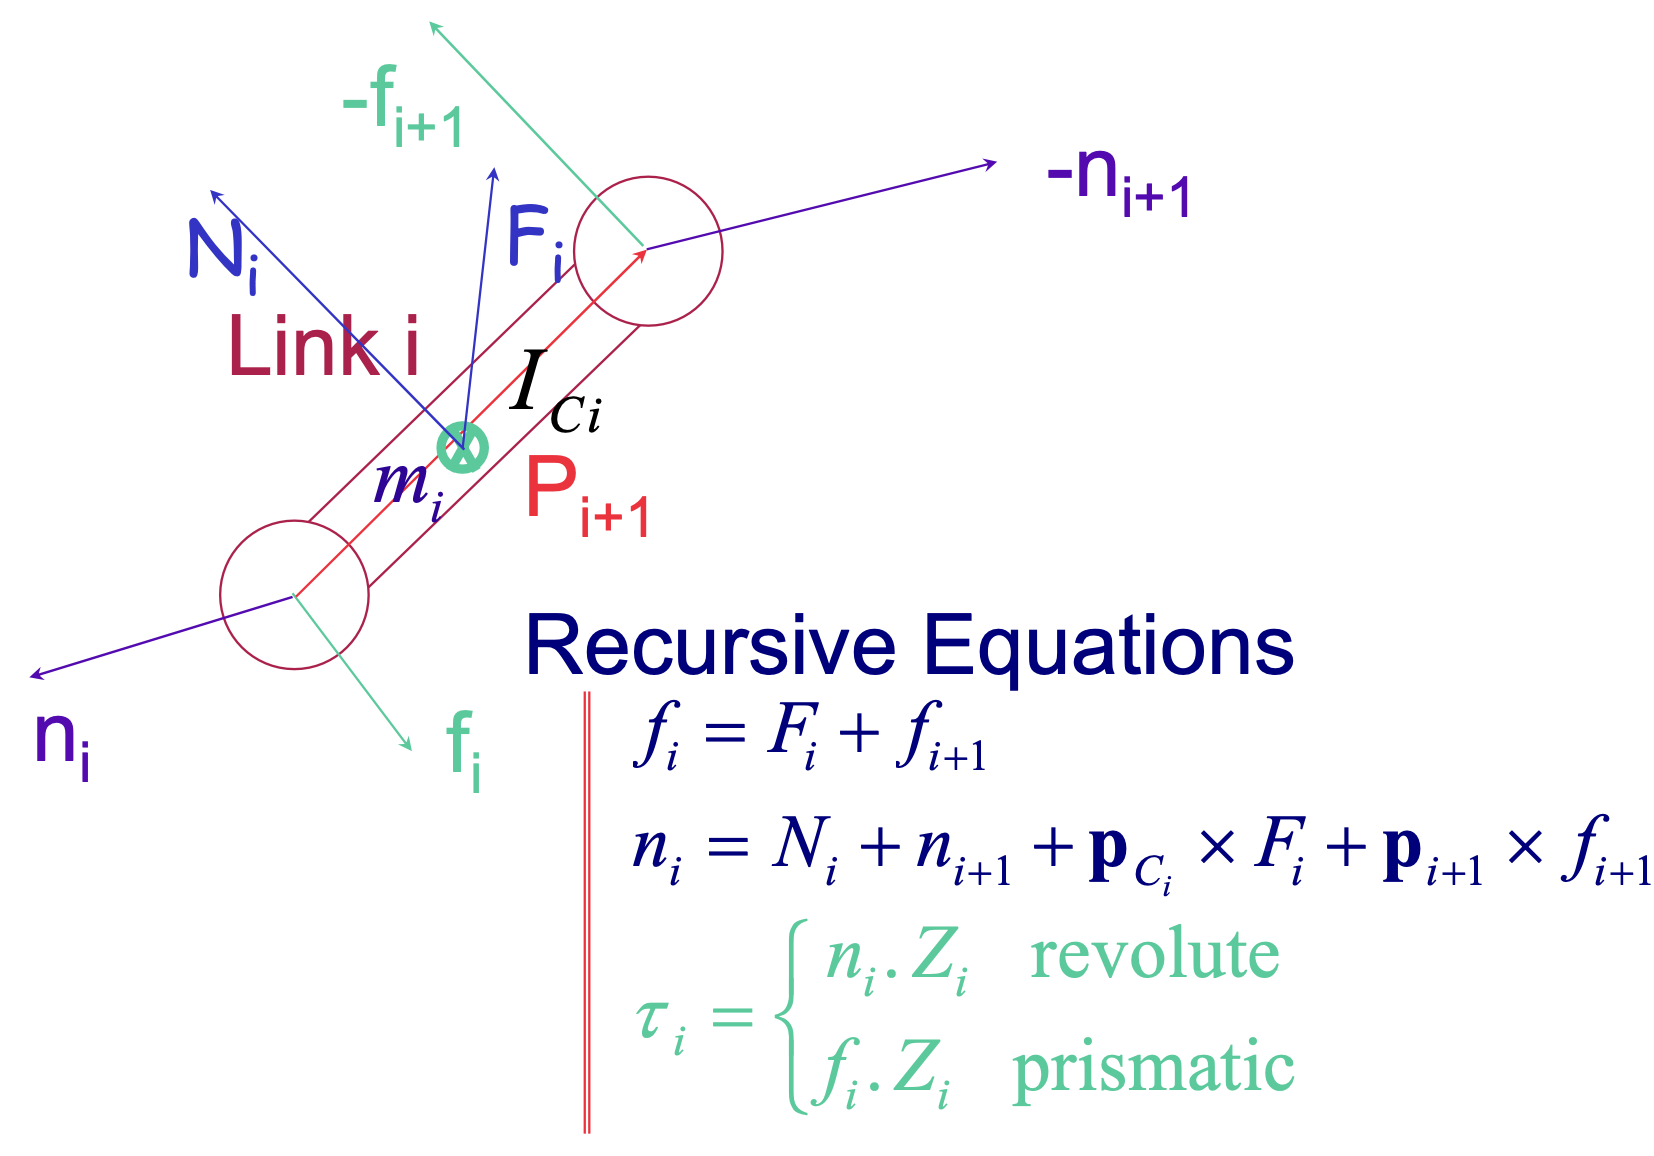
\includegraphics[width=8cm]{sections/imgs/6_newton_euler_recursive_eq.png}
	\hfill
	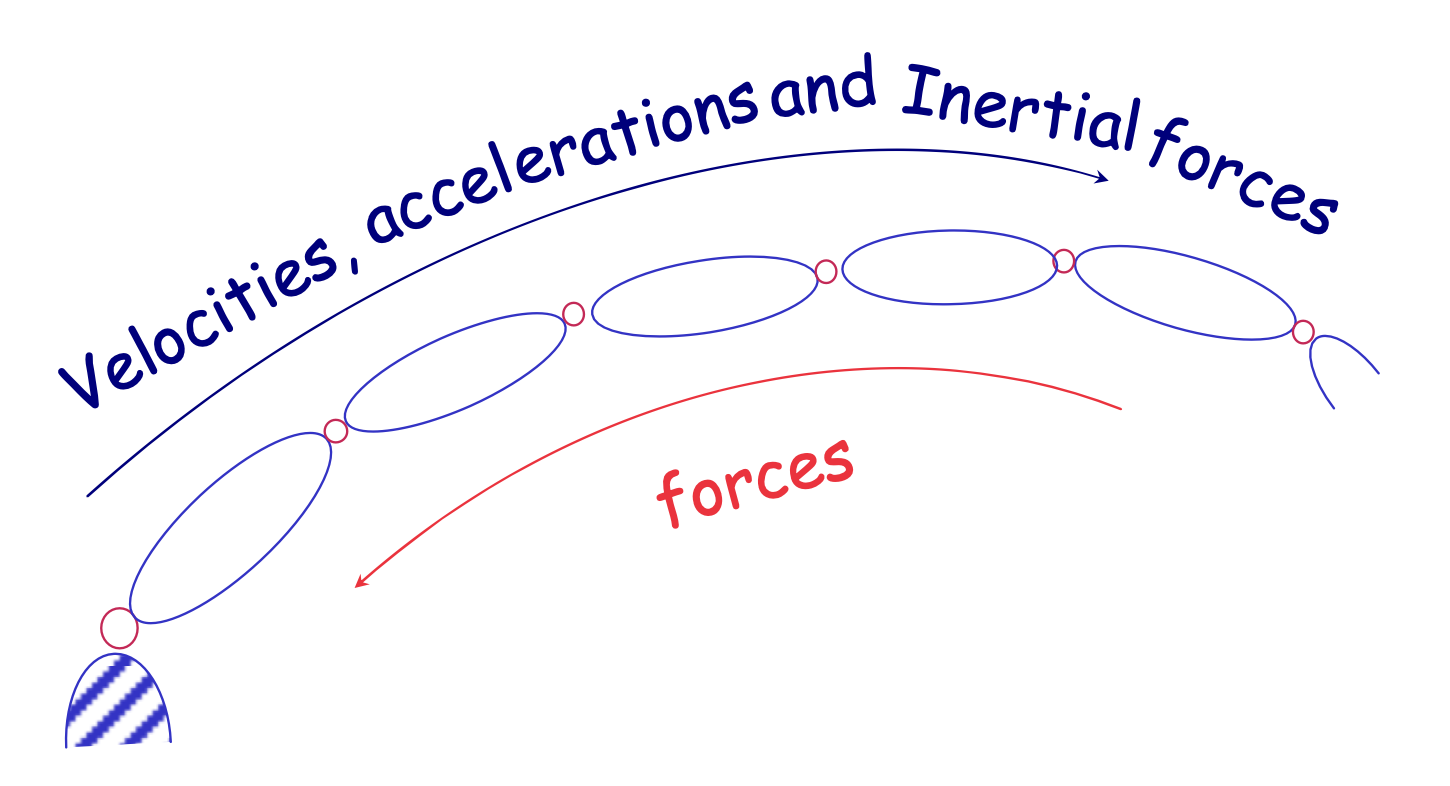
\includegraphics[width=7cm]{sections/imgs/6_newton_euler_alg.png}
\end{center}

If we know the location of the center of mass and the inertia tensor of the link, then its mass
distribution is completely characterised. In order to move the links, we must
We accelerate and decelerate them. The forces required for such motion are a function
of the acceleration desired and of the mass distribution of the links. 

Newton's equation, along with its rotational analog, Euler's equation, describes how forces, inertias, and accelerations relate.

Exercise sheet 4 has a simple examples which demonstrates the Newton-Euler-Algorithm quite well.

\subsection{State-Space equation (M-V-G-form)}

We also need to take into account the effect of gravity on the links of the robot. This can be done by setting ${ }^{0} \dot{v}_{0}=-G$ where $G$ is the gravitational acceleration. We obtain the M-V-G-form by rearranging the equations of movement for the joint torques:

\begin{center}
	$\tau=M(\Theta) \ddot{\Theta}+V(\Theta, \dot{\Theta})+G(\Theta)$
\end{center}

$M$ is a $n\times n$ matrix, and $V$ as well as $G$ are $n\times 1$ vectors. Note that in general, $M$, $V$, $G$ are complex-valued. The matrix $M$ can be determined from the dynamics equations by factorizing all summands that contain  ̈$\ddot{\theta}$. Similarily, $V$ is determined by factorizing all summands that contain $\dot{\theta}$. Finally, $G$ is determined by factorizing all summands that contain $g$. $V$ can be further decomposed into components $B$ and $C$, yielding the configuration-space equation (or M-B-C-G-form):

\begin{center}
	$\tau=M(\Theta) \ddot{\Theta}+B(\Theta)[\dot{\Theta} \dot{\Theta}]+C(\Theta)\left[\dot{\Theta}^{2}\right]+G(\Theta)$
\end{center}

$B(\Theta)$ is a matrix of dimension $n \times n(n-1) / 2$, and $[\dot{\Theta} \dot{\Theta}]$ is an abbreviation for the vector

\begin{center}
	$\left(\dot{\Theta}_{1} \dot{\Theta}_{2}, \dot{\Theta}_{1} \dot{\Theta}_{3}, \ldots, \dot{\Theta}_{n-1} \dot{\Theta}_{n}\right)$
\end{center}

that has length $n(n-1) / 2$. This also explains the dimension of $B$: $n(n-1) / 2$ is the number of products $\Theta_{i} \Theta_{j}$ with $i \neq j$. The matrix $C$ has dimension $n \times n$, and $\left[\dot{\Theta}^{2}\right]$ in an abbreviation for the vector
\begin{center}
$$\left(\dot{\Theta}_{1}^{2}, \dot{\Theta}_{2}^{2}, \ldots, \dot{\Theta}_{n}^{2}\right)^{\mathrm{T}}$$
\end{center}

with length $n$. The matrices $B$ and $C$ can be determined by finding the coefficients of $\Theta_{i} \Theta_{j}$ and $\Theta_{i}^{2}$, respectively.

\subsection{Mass distribution}
In systems with a single degree of freedom, we often talk about the mass of a rigid
body. In the case of rotational motion about a single axis, the notion of the moment
of inertia is a familiar one. 
\subsubsection{Linear Momentum}

The rate of change of the linear momentum for a particle with mass $m$ is equal to the applied force.

\begin{center}
$\begin{aligned}
	\frac{d}{d t}(m v) &= F \\
	\varphi &= mv
\end{aligned}$
\end{center}

\subsubsection{Angular Momentum}
...is the total moment of the momentum of a rigid body's constituting particles:
\[ H_c = \int\limits_{\mathcal{B}}^{} r \times x \mathop{d m} = {}^{A}\mathbf{I} \omega  \]

Angular momentum can be understood as the cross-product of the linear momentum $mv$ and a position vector $p$. This follows from the fact that the rate of change of the angular momentum is equal to the applied moment, hence the left image below. For a rigid body (right image), the total angular momentum $\phi$ is the sum of angular momentum for all particles. The velocity is written as $\omega \times p_i$ and the mass is the integral over the density multiplied by the volume.
\begin{center}
	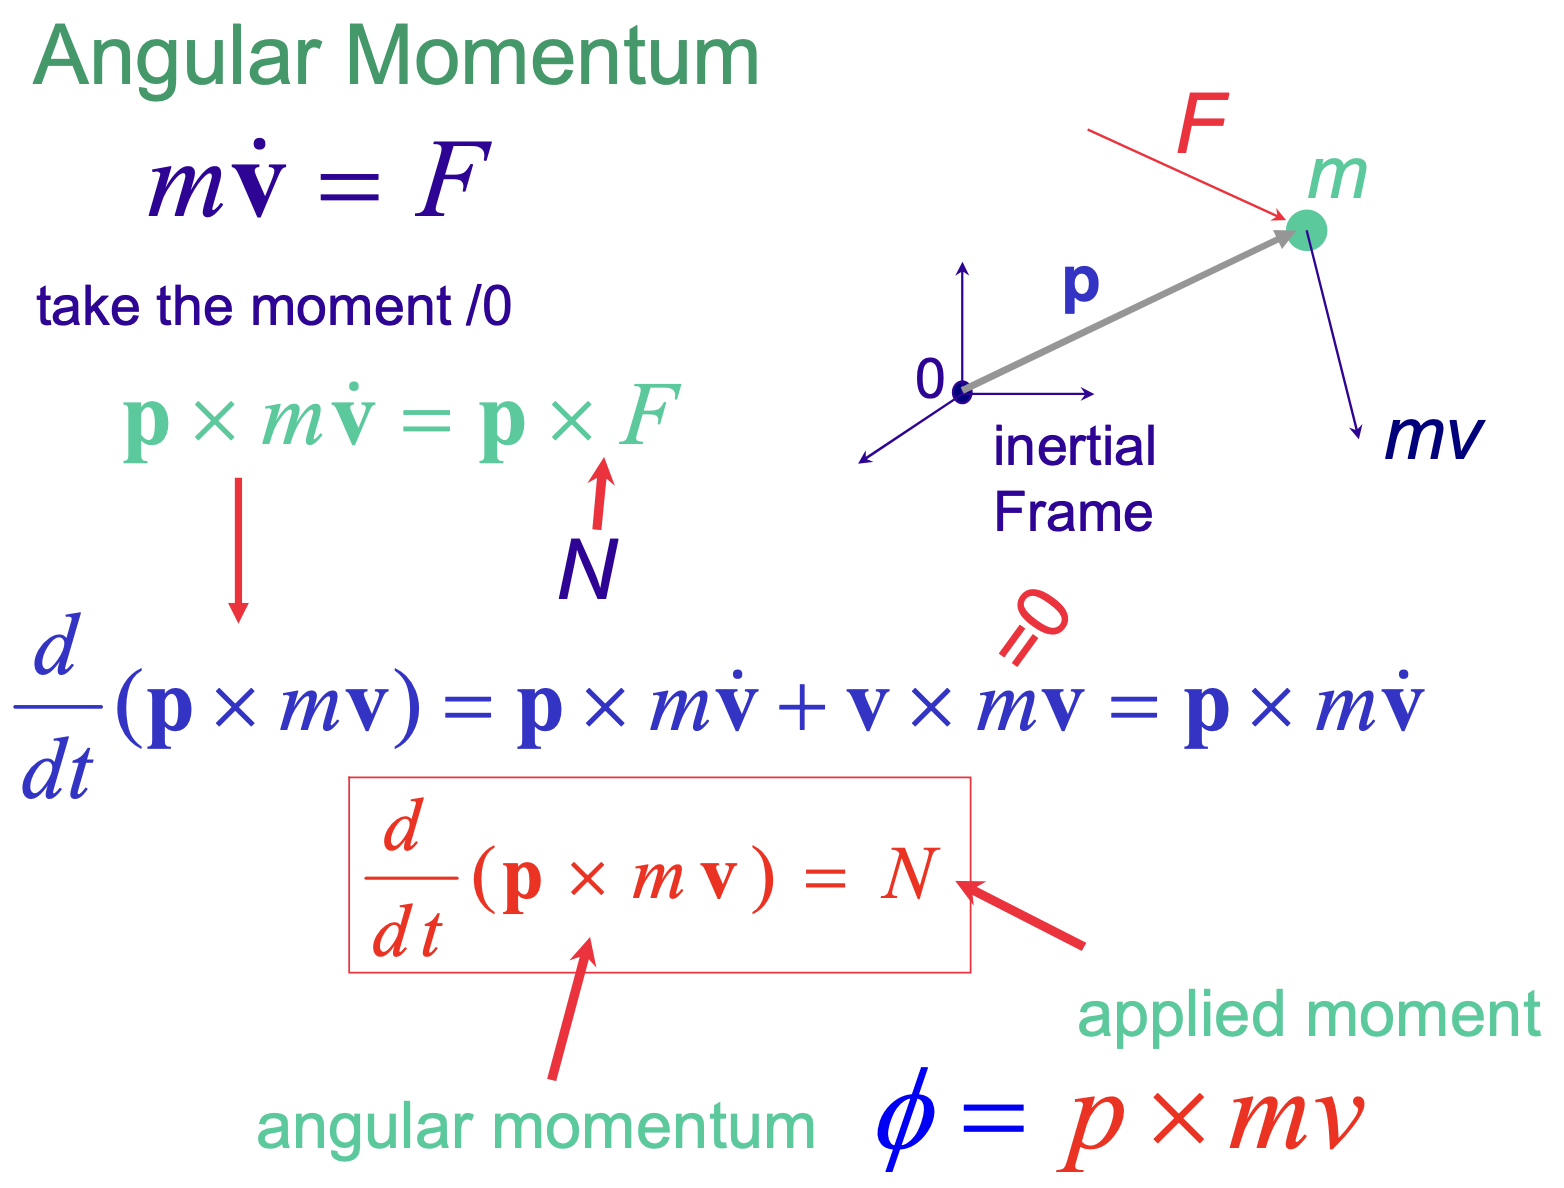
\includegraphics[width=8cm]{sections/imgs/6_angular_momentum.png}
	\hfill
	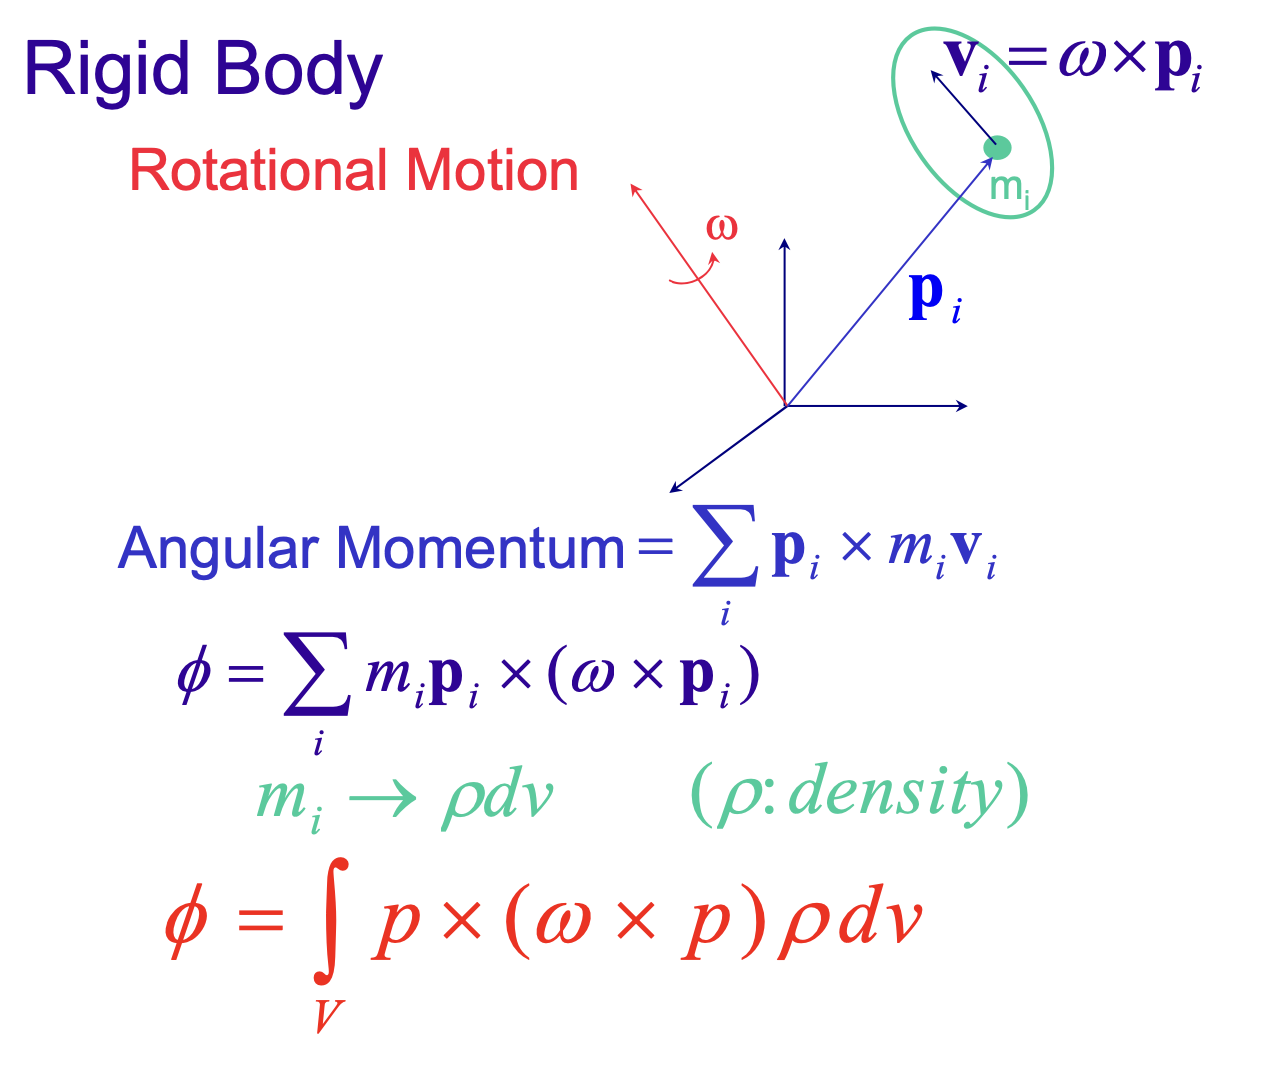
\includegraphics[width=8cm]{sections/imgs/6_rigid_body_angular_momentum.png}
\end{center}

Using the reformulation of the cross-product operator $\mathbf{\hat{p}}=\mathbf{p}\times$ and the fact that $\mathbf{\omega}\times\mathbf{p}=-\mathbf{p}\times\mathbf{\omega}$, wherein $\omega$ is shared among all points, we derive:

\begin{center}
$\begin{aligned}
	\mathbf{p} \times(\omega \times \mathbf{p})&=\hat{\mathbf{p}}(-\hat{\mathbf{p}}) \omega \\
	\phi &= \int_{V} p \times(\omega \times p) \rho d v = \left[\int_{V} -\hat{\mathbf{p}} \hat{\mathbf{p}} \rho d v\right] \omega = \mathbf{I}\omega \\
	\frac{d}{d t}(\mathbf{I} \omega)&=N
\end{aligned}$
\end{center}

\subsubsection{Inertia Tensor}

For a rigid body that is free to move in three dimensions, there are infinitely many possible rotation axes. In the case of rotation about an arbitrary axis, we need a complete way of characterizing the mass distribution of a rigid body. 

The \textbf{inertia tensor} can be
thought of as a generalization of the scalar moment of inertia of an object, relative to the frame attached to the object (rigid body). The left side of the following figure shows the derivation of the inertia tensor from the volume integral of $-\mathbf{\hat{p}}\mathbf{\hat{p}}$. Remember that $\hat{p}$ is the cross-product operator for a point on the rigid body relative to the origin. $I_{xx}, I_{yy}, I_{zz}$ are called \textit{moments of inertia}, while $I_{xy}, I_{xz}, I_{yz}$ are called \textit{products of inertia}.

\begin{center}
\begin{minipage}{0.5\textwidth}
	\begin{center}
		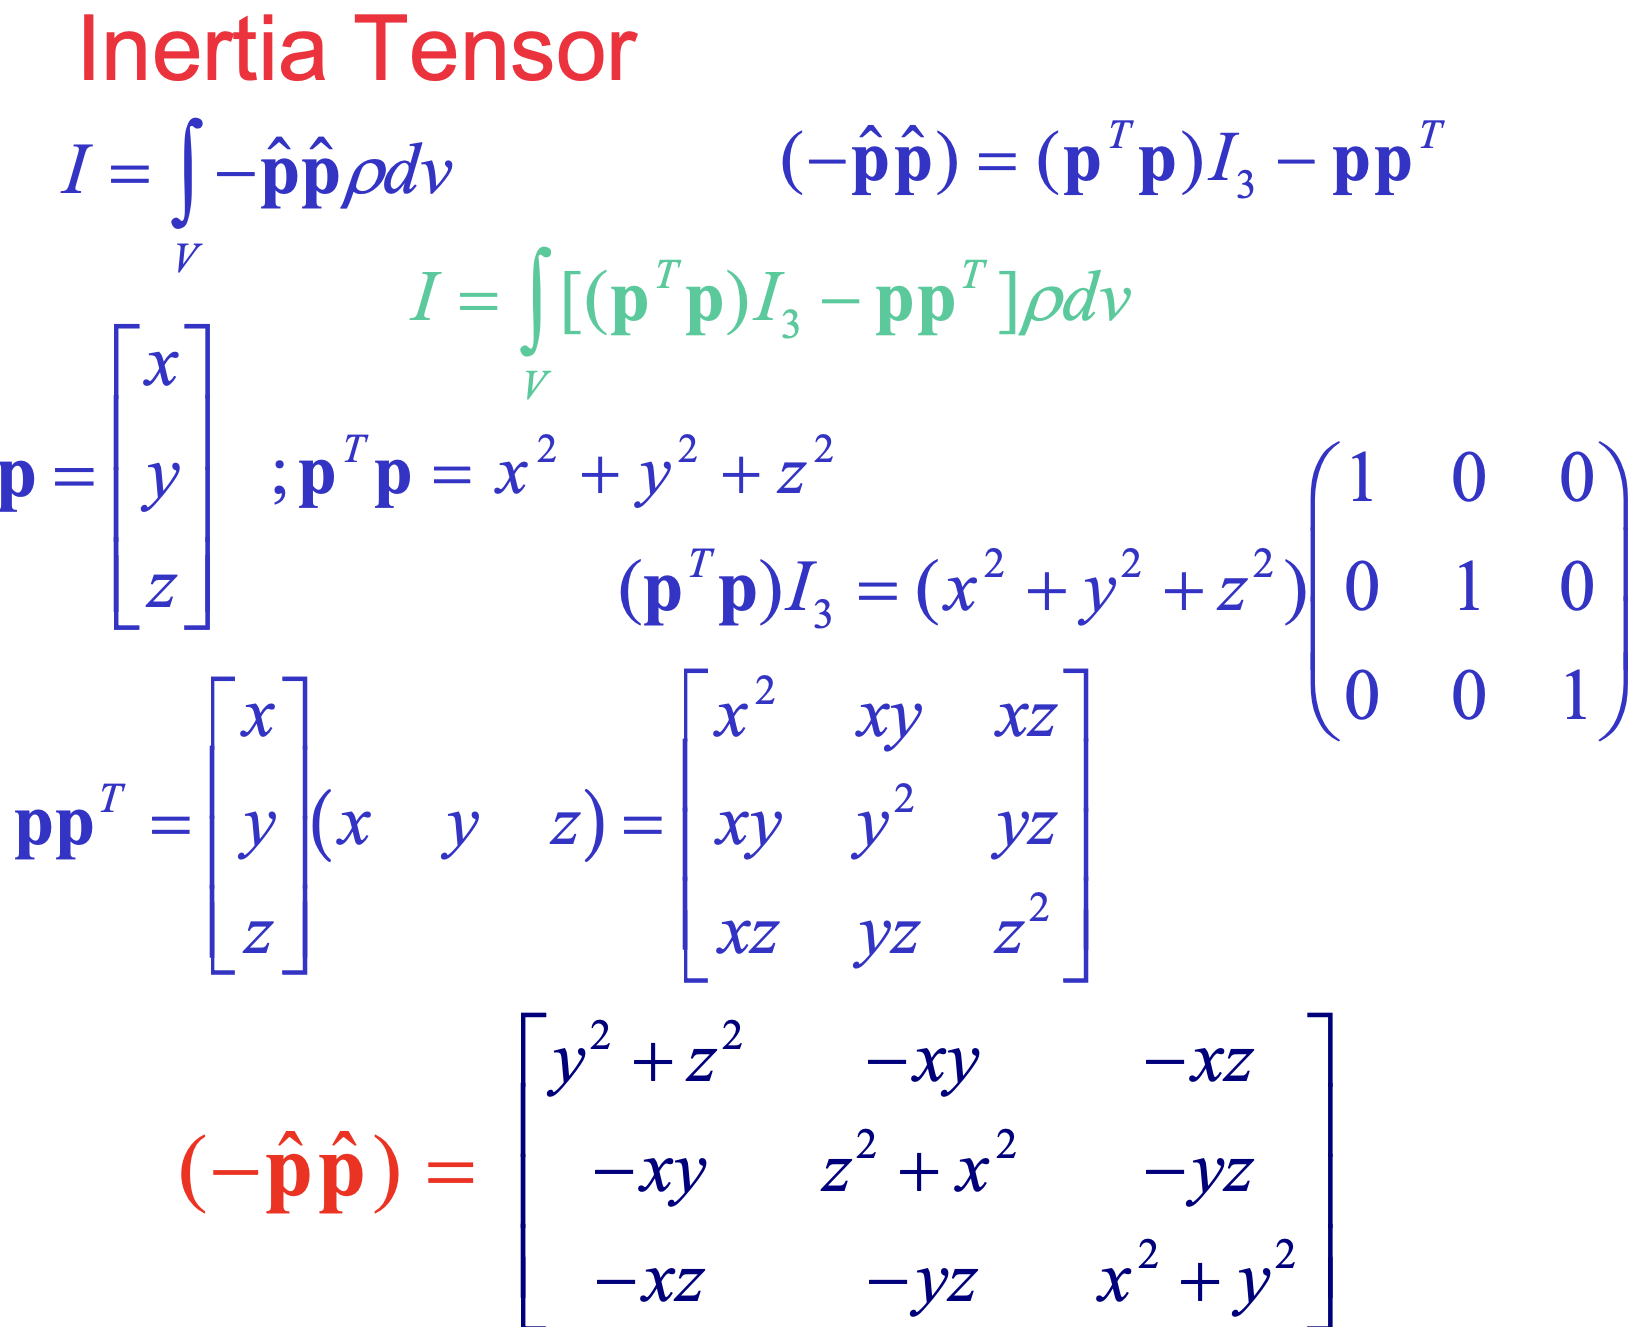
\includegraphics[width=8cm]{sections/imgs/6_inertia_tensor.png}
	\end{center}
\end{minipage}
\begin{minipage}{0.49\textwidth}
	\begin{tabular}{cc}
		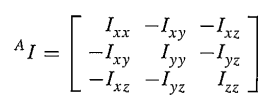
\includegraphics[width=4cm]{sections/imgs/33.png}&\\
		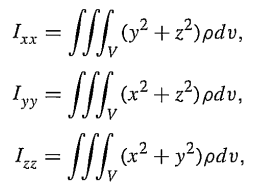
\includegraphics[width=3.5cm]{sections/imgs/34.png}& 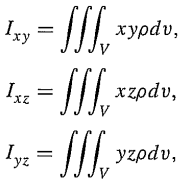
\includegraphics[width=3cm]{sections/imgs/35.png}
	\end{tabular}
\end{minipage}
\end{center}

For an example, check example 6.1 on page 169 or 6.2 on page 171.

\textbf{Some properties:}
\begin{itemize}
	\item Inertia matrices are positive-definite, symmetric matrices.
	\item The inertia matrix is not in general constant and is frame-dependent:
		\[ \mathbf{I}_{c}^{i} = R_{i}^T \mathbf{I}_{c} R_{i} \]
	\item Any rigid body has a set of principal directions with respect to which the inertia matrix is diagonal.
	\item If $xy$ is the plane of symmetry, then $ I_{xz} = I_{yz} = 0 $ (similarly for $xz$ or $yz$).
	\item If the body is axissymmetric (e.g. symmetric about $z$), then the inertia matrix is diagonal and 2 of the moments of inertia equal (e.g. $ I_{xx} = I_{yy} $ if z is axis of symmetry)
\end{itemize}

\subsubsection{Parallel-Axis Theorem}
... is a way of computing how the inertia tensor changes under \textit{translations} of the reference coordinate system (s.t. the axes remain parallel). It relates the inertia tensor in a frame with origin at the center of mass ${}^CI$ to the inertia tensor with respect to another reference frame ${}^AI$. $C$ is located at the center of mass of the body, and $A$ is an arbitrarily translated frame. The theorem can be stated as:
\begin{align*} \label{eq:pat}
	{}^{A} I_{zz} &= {}^{C} I_{zz} + m (x_{c}^2 + y_{c}^2) \\
	{}^{A} I_{xy} &= {}^{C} I_{xy} - m x_{c} y_{c} 
\end{align*}
Where $ P_{c} = [x_{c} , y_{c} , z_{c}]^T $ locates the center of mass relative to $A$. The remaining moments and products of inertia are computed from permutations of $ x,y,z $. The theorem in vector-matrix form:
\[ {}^{A} I = {}^{C} I + m [P_{c}^T P_{c} I_{3} - P_{c} P_{c}^T] \]
with $ I_{3} $ as the identity matrix. The left side of the following image shows the new reference frame $A$ and the center of mass $m$, as well as the connecting vector $P_{c}$.

\begin{center}
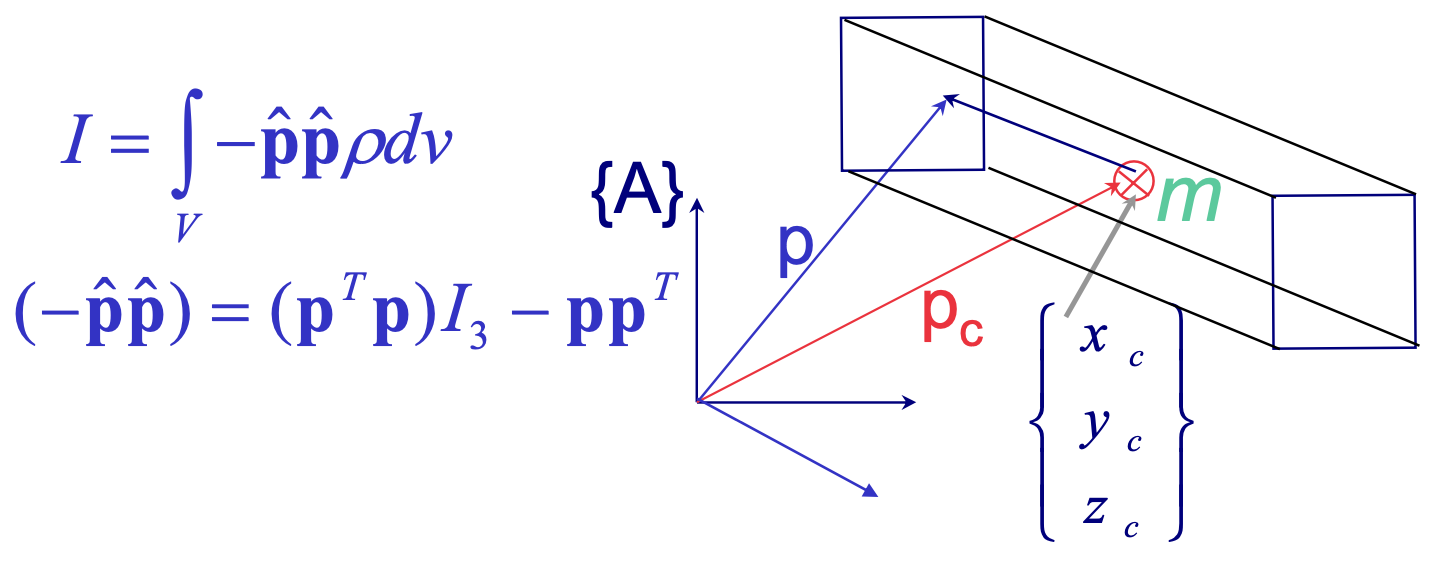
\includegraphics[width=7cm]{sections/imgs/6_parallel_axes.png}
\hfill
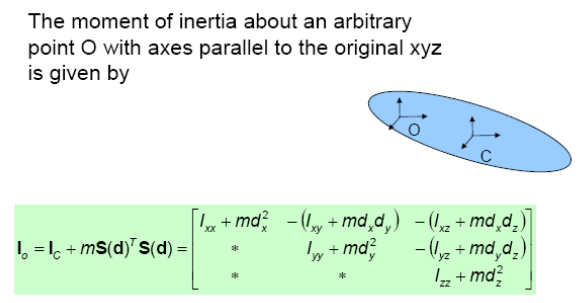
\includegraphics[width=8cm]{sections/imgs/38.png}
\end{center}


\subsection{Euler-Lagrange Equations}

The Lagrangian dynamic formulation is another method for determining the dynamics of a robot which is derived from energy considerations. The Lagrange equation is:

\begin{center}
	$\frac{d}{dt} \frac{\partial L}{\partial \dot{\Theta}} - \frac{\partial L}{\partial \Theta} = \tau$
\end{center}

where the Lagrangian $L=k-u$ is the difference between the kinetic energy $k$ and the potential energy $u$. Since $U=U(\Theta)$, the equation simplifies to

\begin{center}
	$\tau=\frac{d}{d t} \frac{\partial k}{\partial \dot{\Theta}}-\frac{\partial k}{\partial \Theta}+\frac{\partial u}{\partial \Theta}$.
\end{center}

The derivatives of the Lagrange equation are given the left part of the figure below. We set $G=\frac{\partial u}{\partial \Theta}$ since it only depends on $\Theta$. By calculating the derivatives, we see that the Lagrange equation is in M-V-G-form. Next, we can identify $M(q)$ from the expression $k=\frac{1}{2} \dot{q}^{T} M \dot{q}$. With knowledge of $M$ the expression in pink gives us $V(q, \dot{q})$.
\\

\begin{minipage}[c]{0.5\textwidth}
	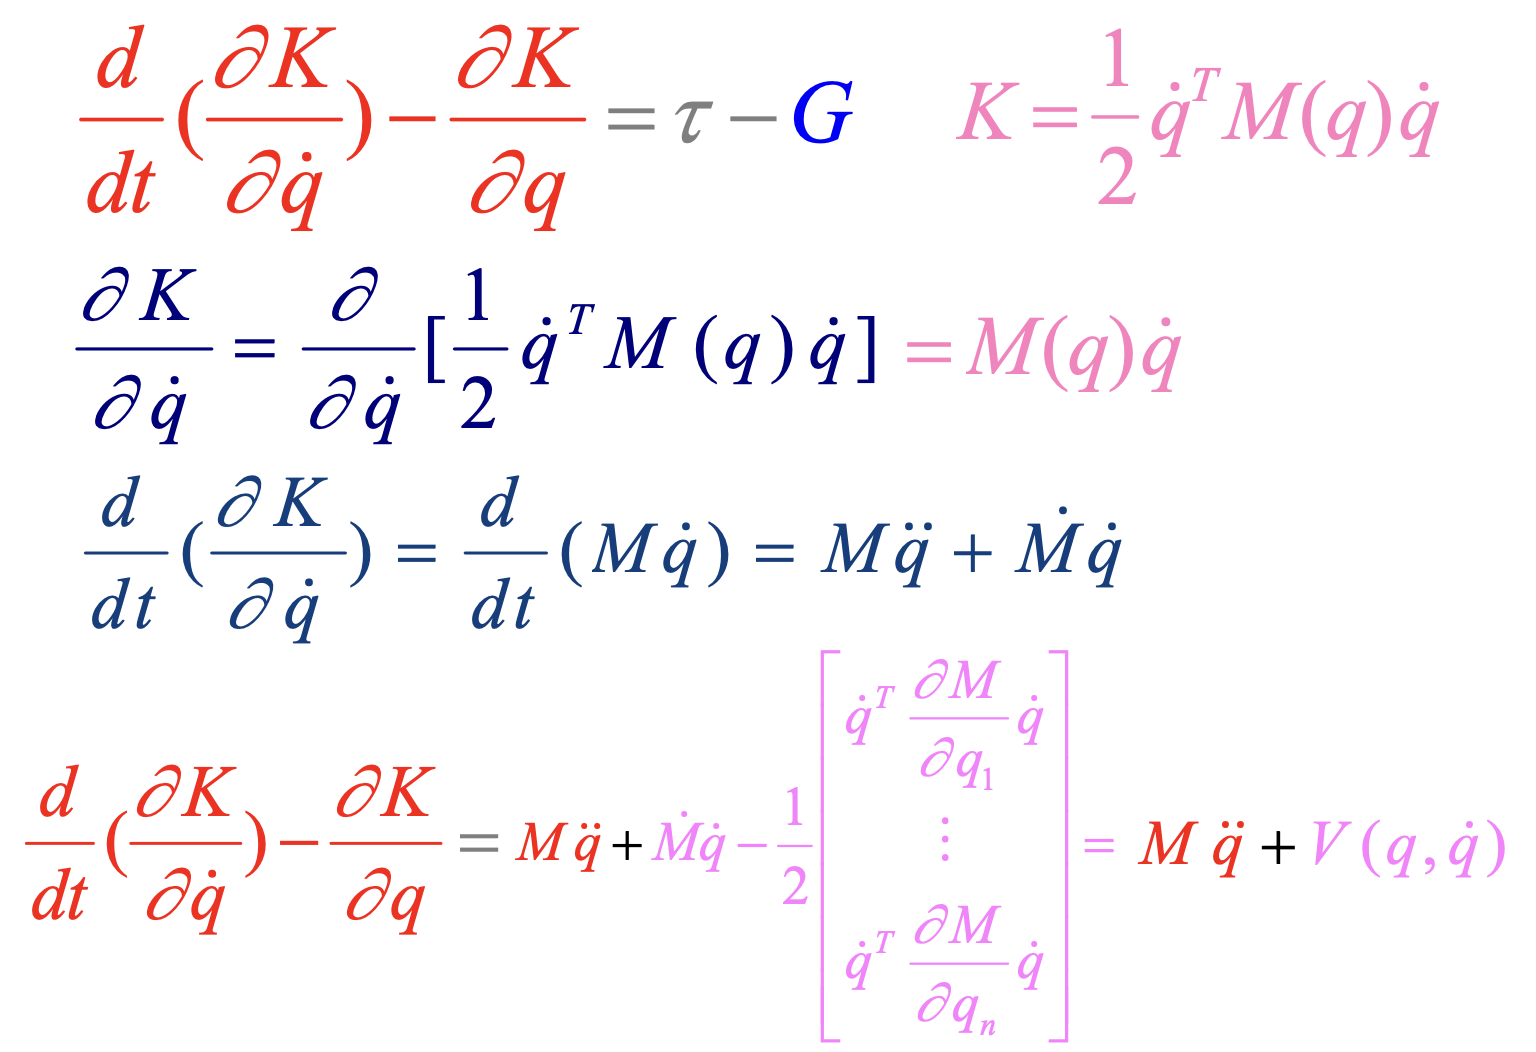
\includegraphics[width=9cm]{sections/imgs/6_lagrange_mvg.png}
\end{minipage}
\hfill
\begin{minipage}[c]{0.5\textwidth}
\begin{center}
	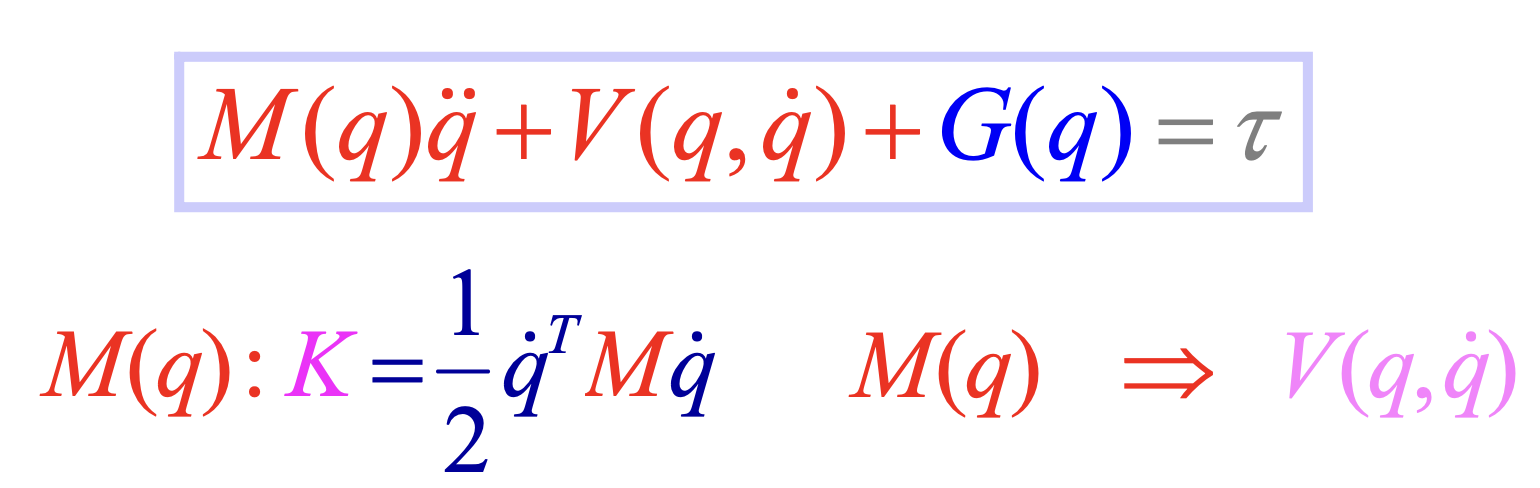
\includegraphics[width=6cm]{sections/imgs/6_lagrange_vmg_2.png}
\end{center}

\end{minipage}

For each link of the robot, the kinetic energy can be computed as (and is the same for any reference frame of the velocities):

\begin{center}
	$k_{i}=\frac{1}{2} m_{i} v_{C_{i}}^{\mathrm{T}} \cdot v_{C_{i}}+\frac{1}{2} {}^i \omega_{i}^{\mathrm{T}} \cdot{ }^{C_{i}} I_{i} \cdot{ }^{i} \omega_{i}$
\end{center}

The first term corresponds to the kinetic energy caused by the linear motion of the link, and the second term corresponds to the kinetic energy caused by the rotational velocity of the link. To determine these energies, we need to compute the linear and rotational velocities of the joints. The overall kinetic energy computes then as sum of the kinetic energies of all links:

\begin{center}
	$k=\sum_{i=1}^{n} k_{i}$
\end{center}

Another way to compute kinetic energy is

\begin{center}
	$k(\Theta, \dot{\Theta})=\frac{1}{2} \dot{\Theta}^{\mathrm{T}} M(\Theta) \dot{\Theta}$
\end{center}

where $M$ again is the $n\times n$ mass matrix from the M-V-G form of the dynamics equations. By setting both formulas for $k$ equal to each other and expressing the velocities at the centres of mass with their Jacobians, we derive an expression for $M$, as the next figure shows. Note that these Jacobians relate the joint parameters to the velocities at the centres of mass of each link instead of at the joints. As shown in the bottom right corner, they only regard these relations up to the link $i$. All columns after this point are zero.
\\

\begin{minipage}[c]{0.5\textwidth}
	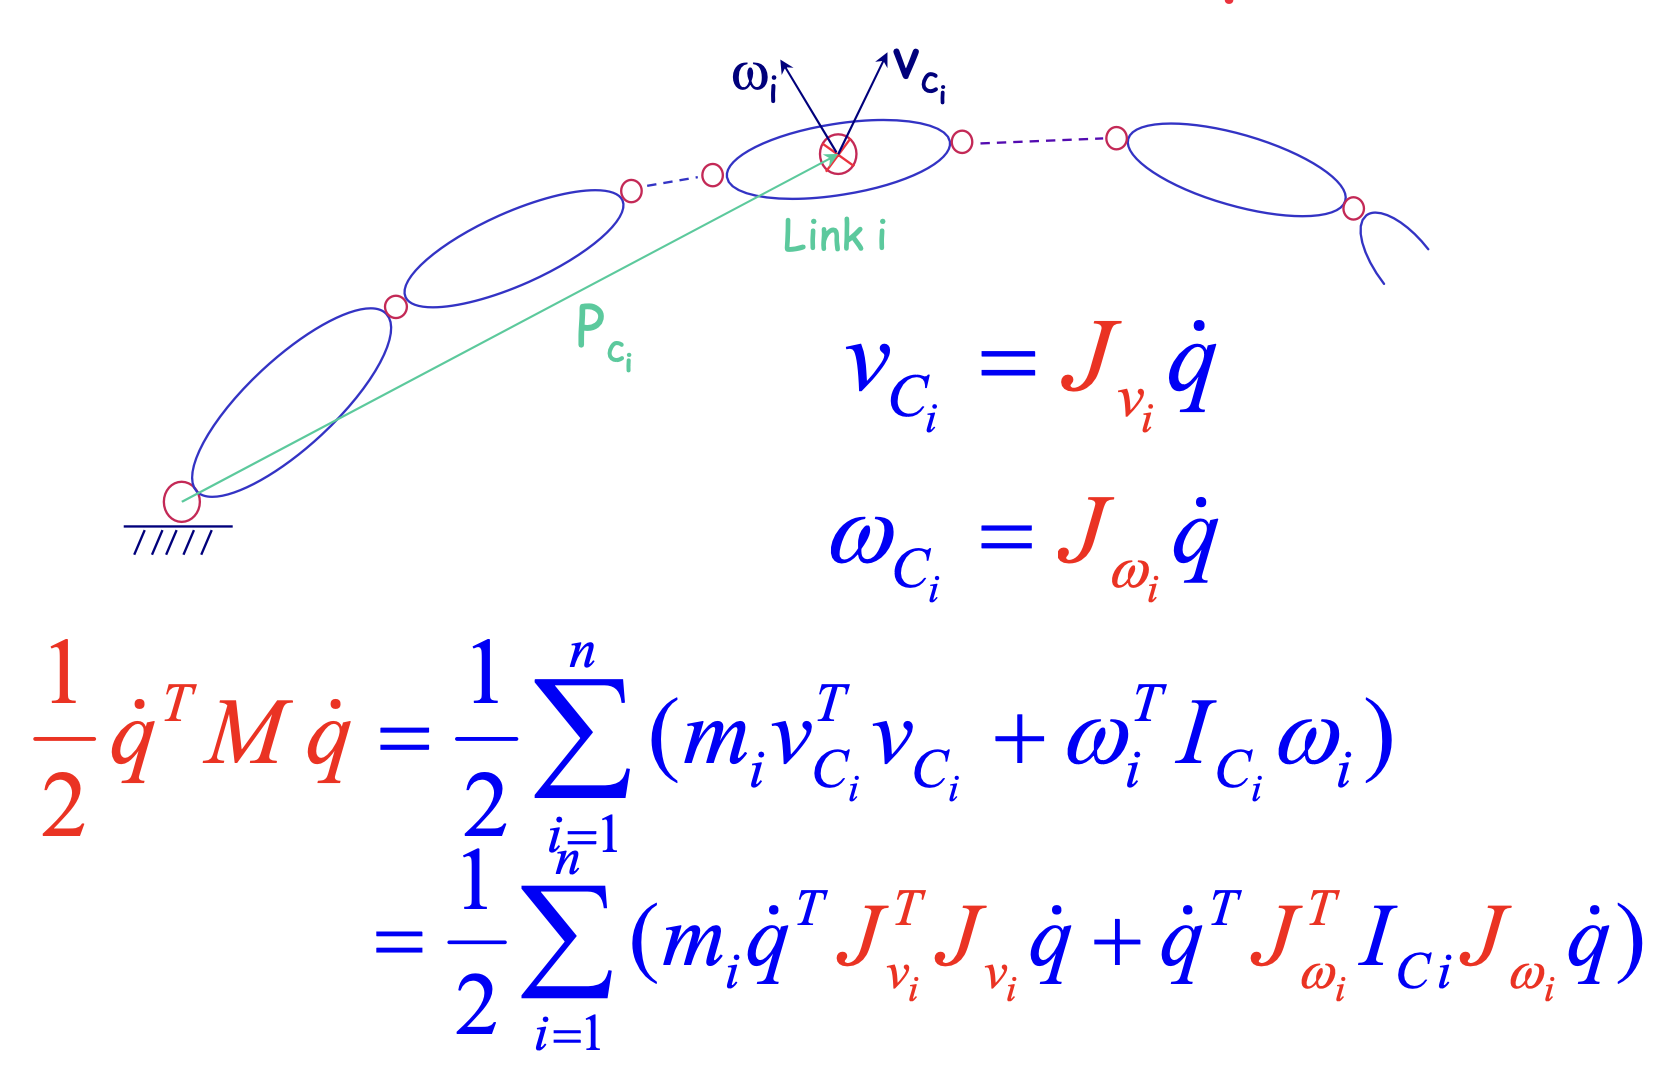
\includegraphics[width=9cm]{sections/imgs/6_mass_matrix_jacobian.png}
\end{minipage}
\hfill
\begin{minipage}[c]{0.5\textwidth}
\begin{center}
	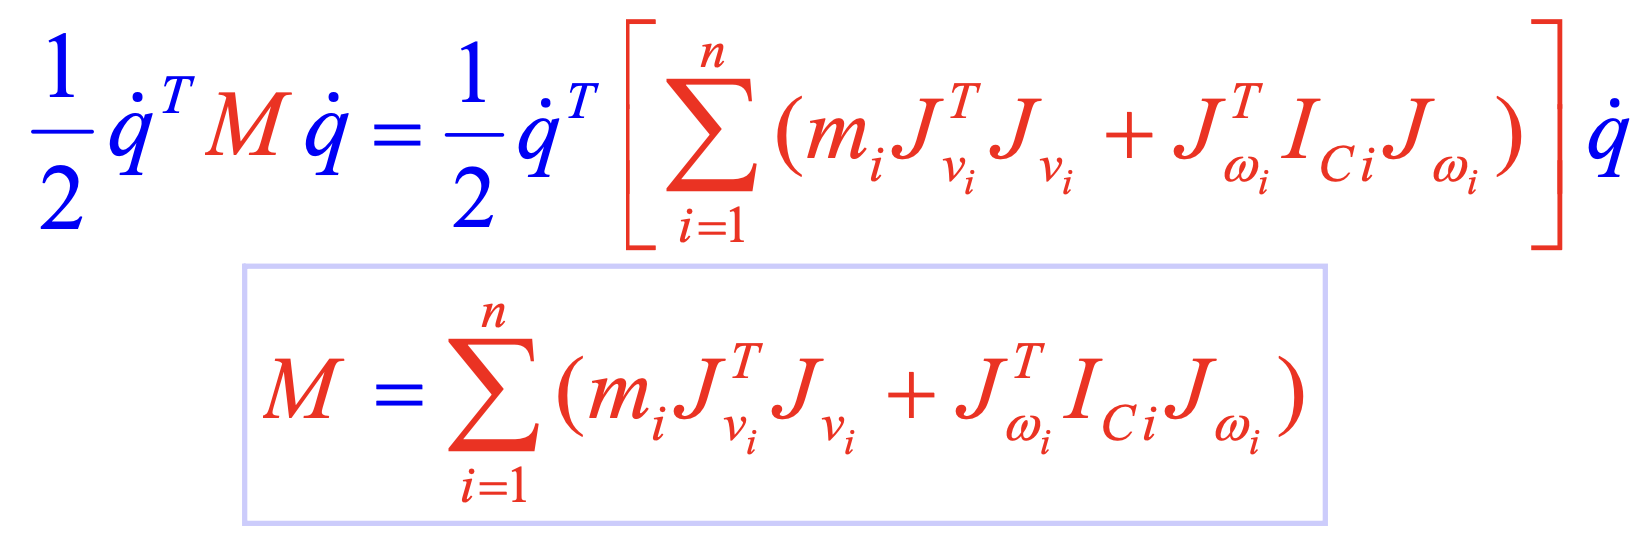
\includegraphics[width=7cm]{sections/imgs/6_mass_matrix_jacobian_2.png}
	\vfill
	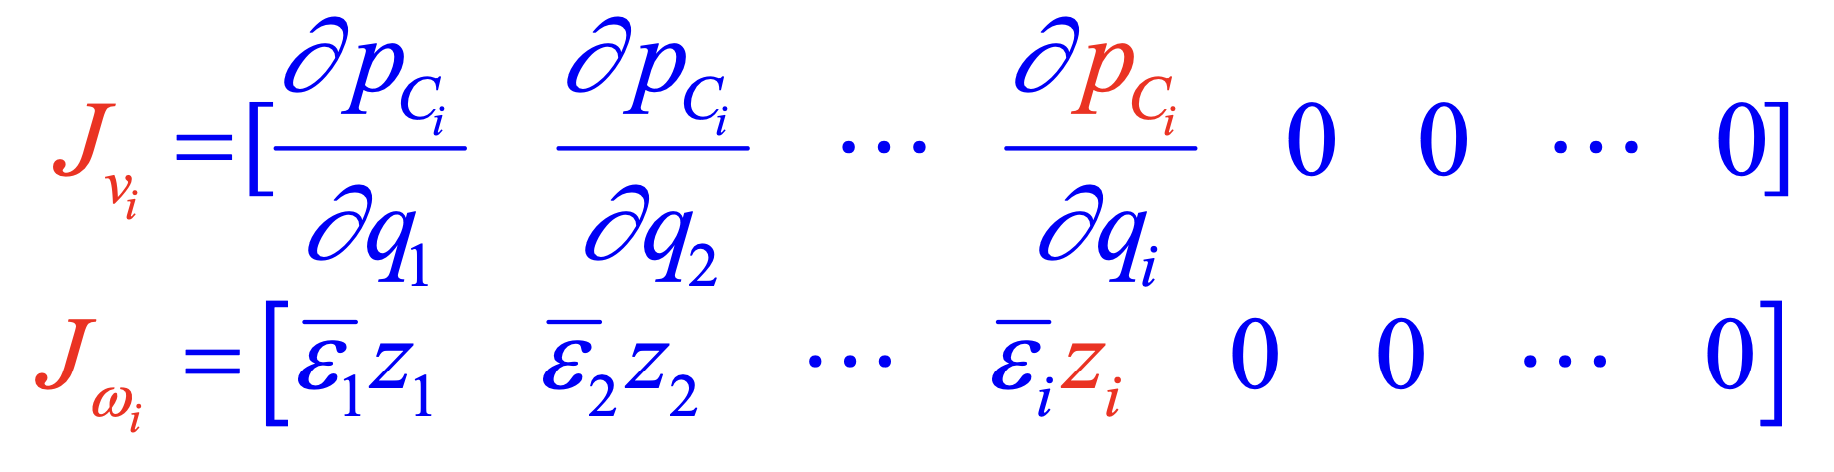
\includegraphics[width=7cm]{sections/imgs/6_mass_matrix_jacobian_3.png}
\end{center}
\end{minipage}

To compute all energies that are present in this system, we also need to take into account the potential energy:

\begin{center}
	$u_{i}=-m_{i} \cdot{ }^{0} g^{\mathrm{T}} \cdot{ }^{0} P_{C_{i}}+u_{\mathrm{ref}_{i}}$
\end{center}

Here, $g$ is the vector of gravity, ${ }^{0} P_{C_{i}}$ denotes the centre of mass of link $i$, and $u_{\mathrm{ref}_{i}}$, is an arbitrary constant (the constant is added because potential energy depends on height, and a certain base height can be chosen arbitrarily). In the further computations, this constant will not play a role, since only the derivatives of the potential energy are considered - and any constant will vanish when differentiated. 
By differentiating the potential energy, we obtain the gravity vector $G$, which also contains the Jacobians. Thus, another way to think of the gravity vector is as the torque in each joint that is caused by a force pulling down on every link of the robot. This is shown in the right part of the figure below.

\begin{center}
	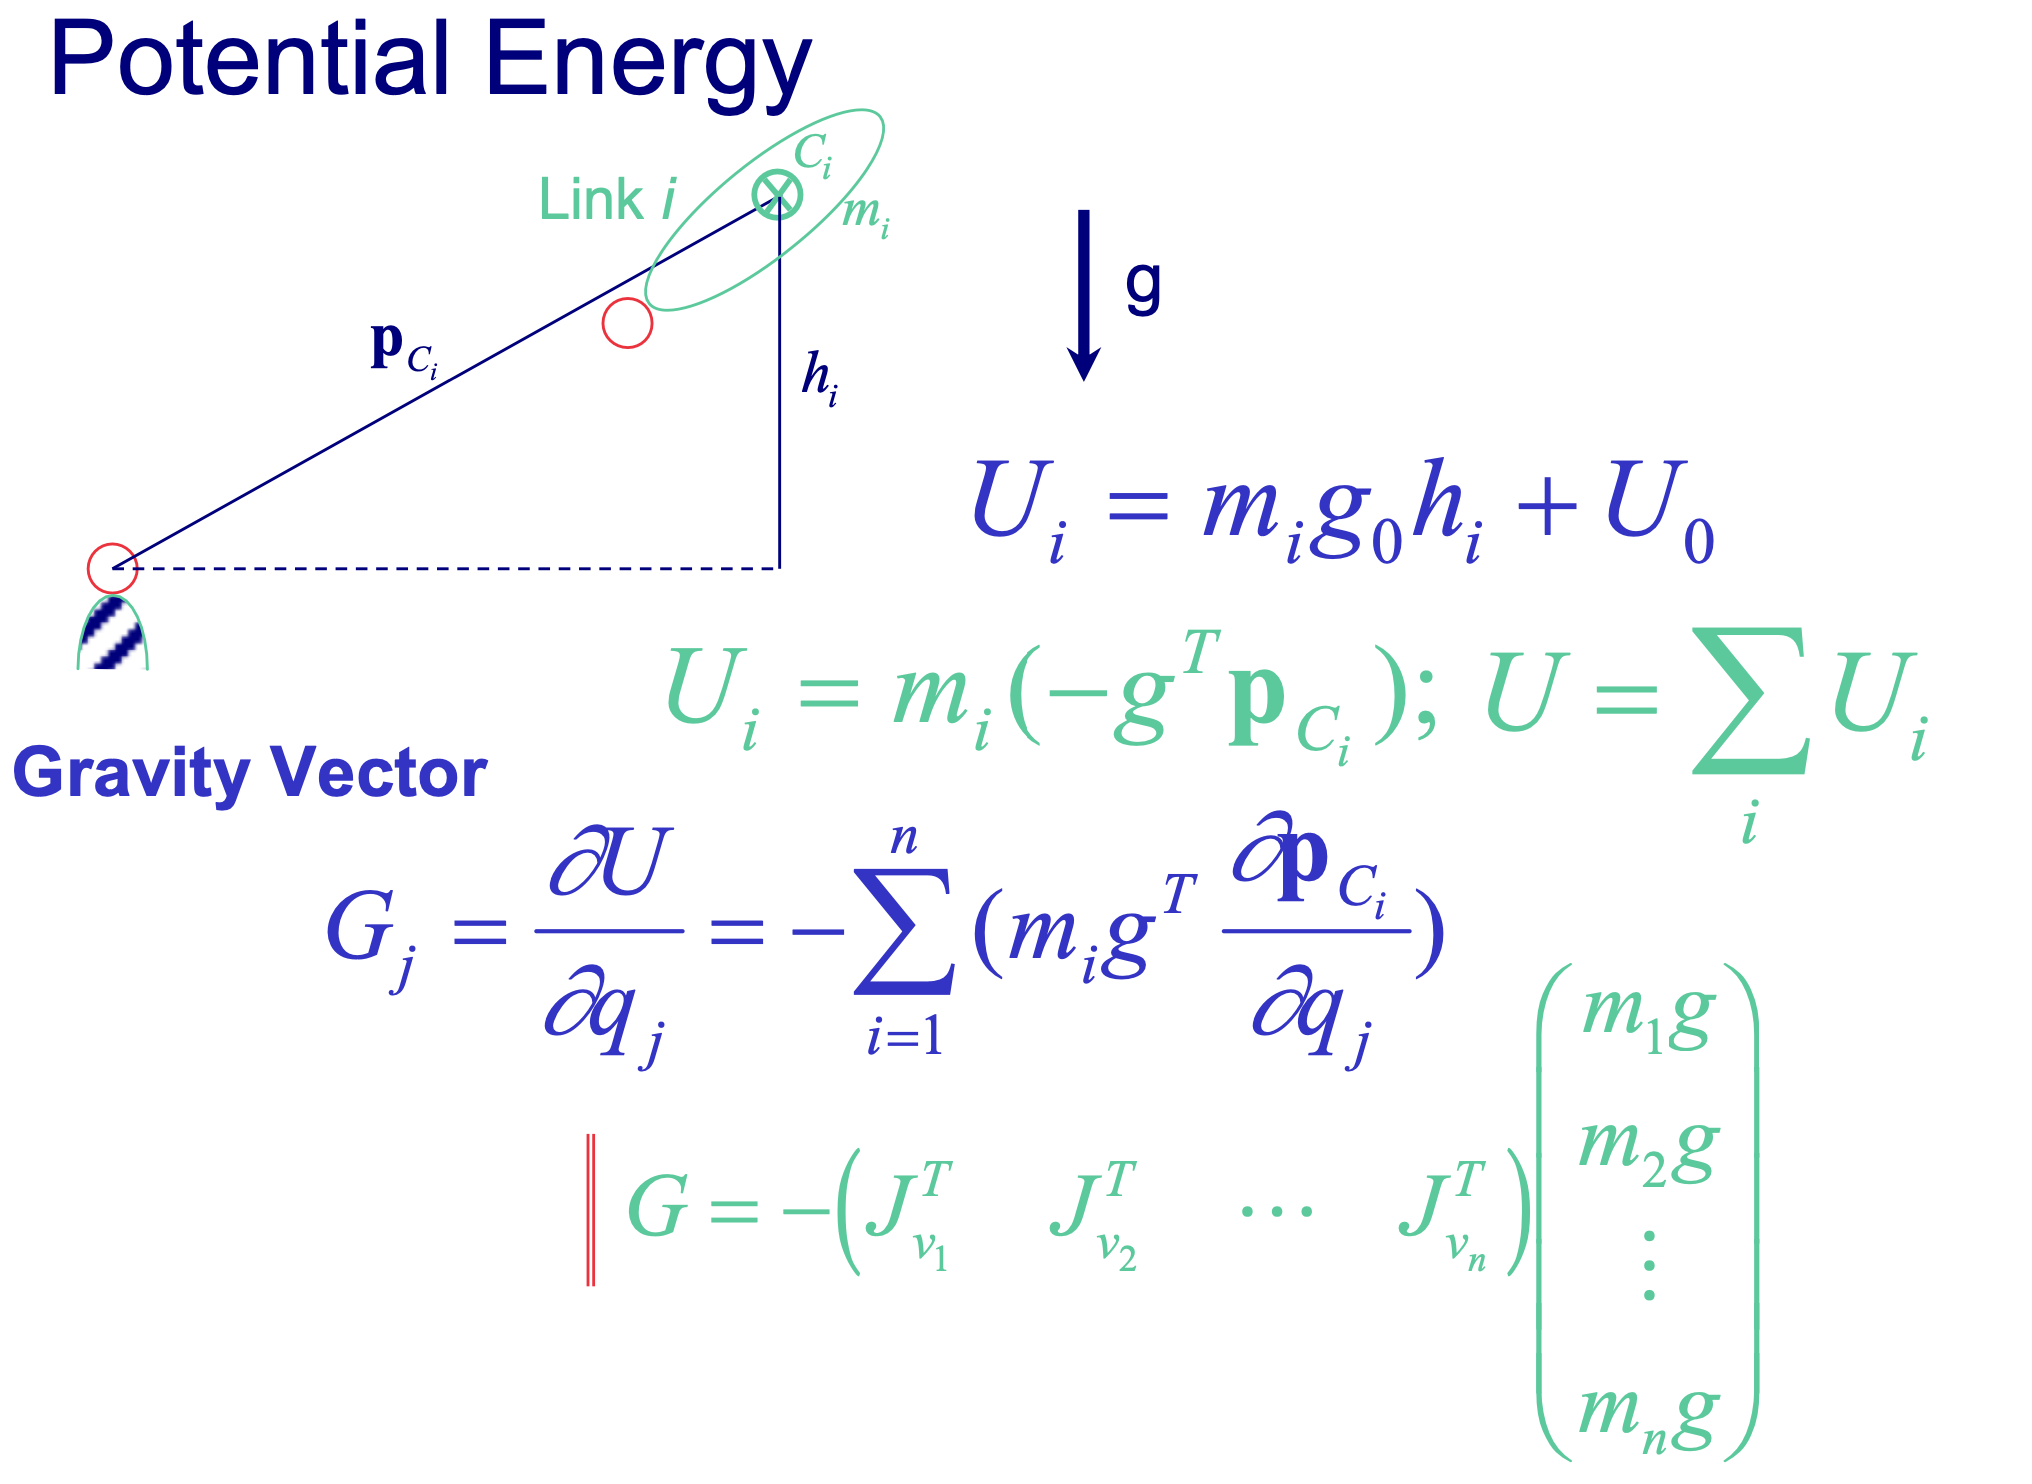
\includegraphics[width=8cm]{sections/imgs/6_lagrange_potential_energy.png}
	\hfill
	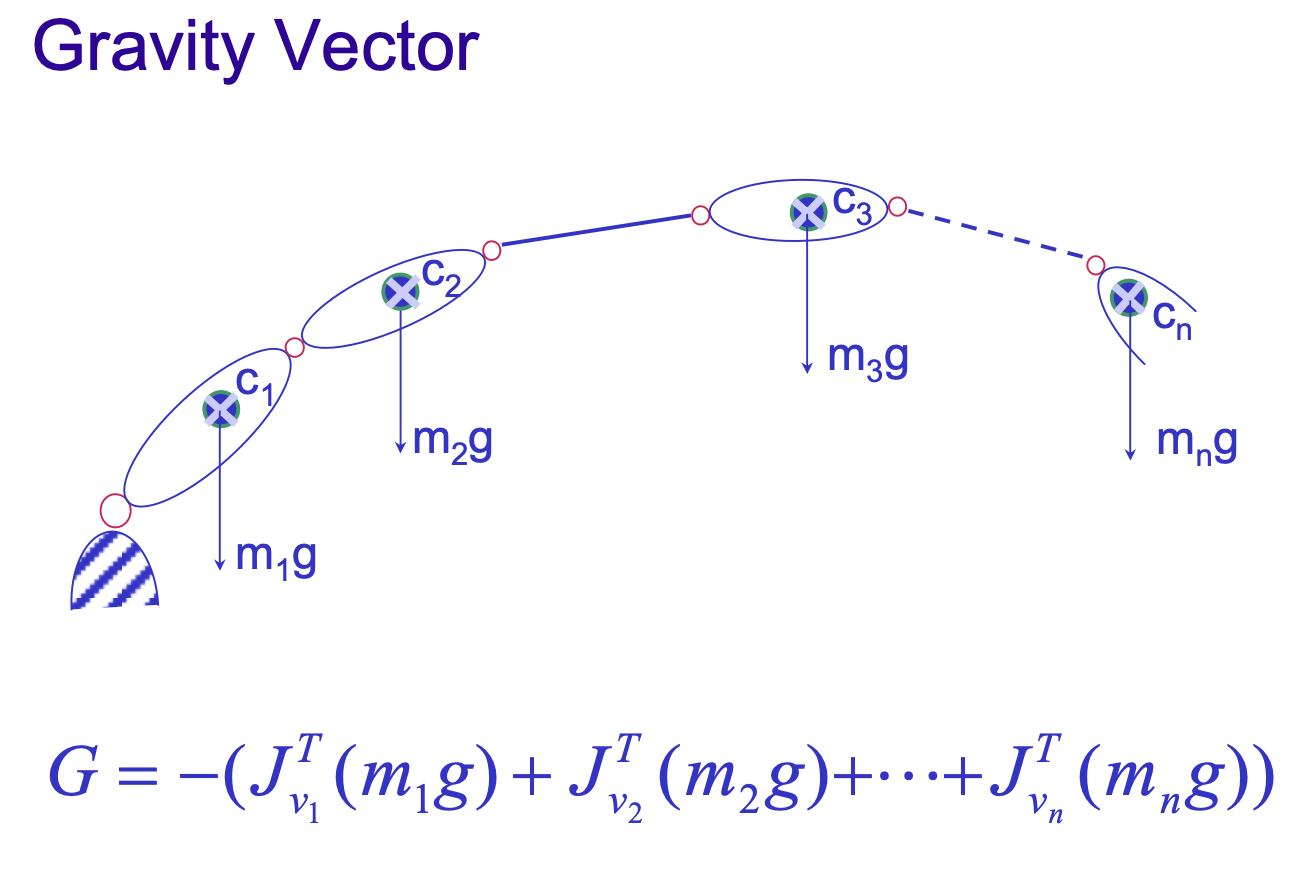
\includegraphics[width=7cm]{sections/imgs/6_lagrange_potential_energy_2.png}
\end{center}

The computation of $\tau$ is finally done through the following formula:

\begin{center}
	$\tau=\frac{d}{d t} \frac{\partial k}{\partial \dot{\Theta}}-\frac{\partial k}{\partial \Theta}+\frac{\partial u}{\partial \Theta}$
\end{center}

It is also possible to compute the joint torques τi on a per-joint basis, which is more practical in most cases. The formula then becomes:

\begin{center}
	$\tau_{i}=\frac{d}{d t} \frac{\partial k}{\partial \dot{\Theta}_{i}}-\frac{\partial k}{\partial \Theta_{i}}+\frac{\partial u}{\partial \Theta_{i}}$
\end{center}